% !TEX program = xelatex
\documentclass[12pt]{article}
\usepackage{iftex}
\ifPDFTeX
    \usepackage[T2A]{fontenc}
    \usepackage[utf8]{inputenc}
\else
    \usepackage{fontspec}
    \IfFontExistsTF{CMU Serif}
        {\setmainfont{CMU Serif}}
        {\IfFontExistsTF{Times New Roman}
            {\setmainfont{Times New Roman}}
            {\setmainfont{TeX Gyre Termes}}}
\fi
\usepackage[russian]{babel}
\usepackage{amsmath}
\usepackage{amssymb}
\usepackage{graphicx}
\usepackage{float}
\usepackage{array}
\usepackage{geometry}
\usepackage{hyperref}

\geometry{left=3cm, right=3cm, top=2cm, bottom=2cm}
\hypersetup{colorlinks=true, linkcolor=black, citecolor=black, urlcolor=black}
\sloppy

\begin{document}

\begin{titlepage}
    \centering
    {\large Московский физико-технический институт\\[0.3cm]
    Физтех-школа природоподобных, плазменных и ядерных технологий им. И.В. Курчатова\\[0.3cm]
    Кафедра моделирования ядерных процессов и технологий\par}

    \vspace{2.5cm}

    {\Large\bfseries Магистерская дипломная работа\par}

    \vspace{1.5cm}

    {\LARGE\bfseries Двухканальная модель памяти твэла: доплеровский и тепловой отклик импульса мощности\par}

    \vspace{2.5cm}

    \begin{flushright}
        \begin{tabular}{>{\raggedleft\arraybackslash}p{5cm}p{7cm}}
            Выполнил: & студент группы М07-405\\
            & Елесин Георгий Павлович\\[0.4cm]
            Направление: & 03.04.01 Прикладные математика и физика\\[0.4cm]
            Профиль: & Общая и прикладная физика\\[0.4cm]
            Специализация: & Суперкомпьютерное моделирование в прикладной физике\\[0.4cm]
            Научный руководитель: & Цибульский Виктор Филиппович\\
        \end{tabular}
    \end{flushright}

    \vfill

    {Москва, 2026}
\end{titlepage}

\tableofcontents
\newpage

\section{Введение}

Импульсное энерговыделение в ядерном топливе нельзя полностью описать статическим температурным коэффициентом реактивности. В стационарной записи доплеровская обратная связь часто сводится к выражению
\[
\rho_D=\alpha_D\Delta T_f.
\]
Такая форма полезна для малых квазистационарных отклонений, но в коротком переходном процессе температура топлива является не внешним параметром, а результатом предшествующей истории мощности. Поэтому в данной работе твэл рассматривается как динамический элемент памяти: импульс мощности записывает в топливе температурный след, а этот след затем имеет два выхода.

Первый выход является реактивностным. Нагрев топлива уширяет резонансы поглощения тяжёлых изотопов, увеличивает резонансный захват и создаёт отрицательную доплеровскую реактивность \cite{NRCFeedback2012,DOEGeneralTechnicalBase2013}. В предлагаемой постановке этот эффект записывается не как мгновенная функция средней температуры, а как свёртка истории мощности с реактивностным ядром:
\[
\rho_D(t)=
-\int_0^tK_D(t-s)P(s)\,ds.
\]
Второй выход является тепловым. Энергия, депонированная в топливе, не попадает в воду мгновенно: она проходит через топливо, зазор, оболочку и поверхность теплообмена. Поэтому вода видит не сам нейтронный пик, а запаздывающий тепловой поток:
\[
Q_{fw}(t)=
\int_0^tH_{fw}(t-s)P(s)\,ds.
\]
Итак, центральная модель работы имеет вид
\[
P(t)
\longrightarrow
\begin{cases}
I_D(t)=K_D*P, & \text{доплеровская реактивностная память},\\[3pt]
Q_{fw}(t)=H_{fw}*P, & \text{тепловой поток в воду}.
\end{cases}
\]

Цель работы состоит в построении этой двухканальной модели и проверке того, какие её элементы могут быть идентифицированы по расчётам GeN-Foam. Научная новизна состоит в замене статического коэффициента реактивности на геометрически определённое ядро памяти \(K_D(t)\), а также во введении второго ядра \(H_{fw}(t)\), описывающего задержанный тепловой выход к воде.

Важный результат работы является отрицательным в физическом, но положительным в методическом смысле. Рассмотренный GeN-Foam case не является режимом доплеровского самогашения: топливная обратная связь оказывается примерно на три порядка меньше внешней вставки реактивности. Поэтому расчёт используется как weak-coupled benchmark для проверки диагностики. По серии малых импульсов тепловой канал \(H_{fw}\) идентифицируется устойчиво, тогда как реактивностный канал \(K_D\) в данной постановке остаётся ниже уровня надёжного восстановления.

\begin{figure}[H]
\centering
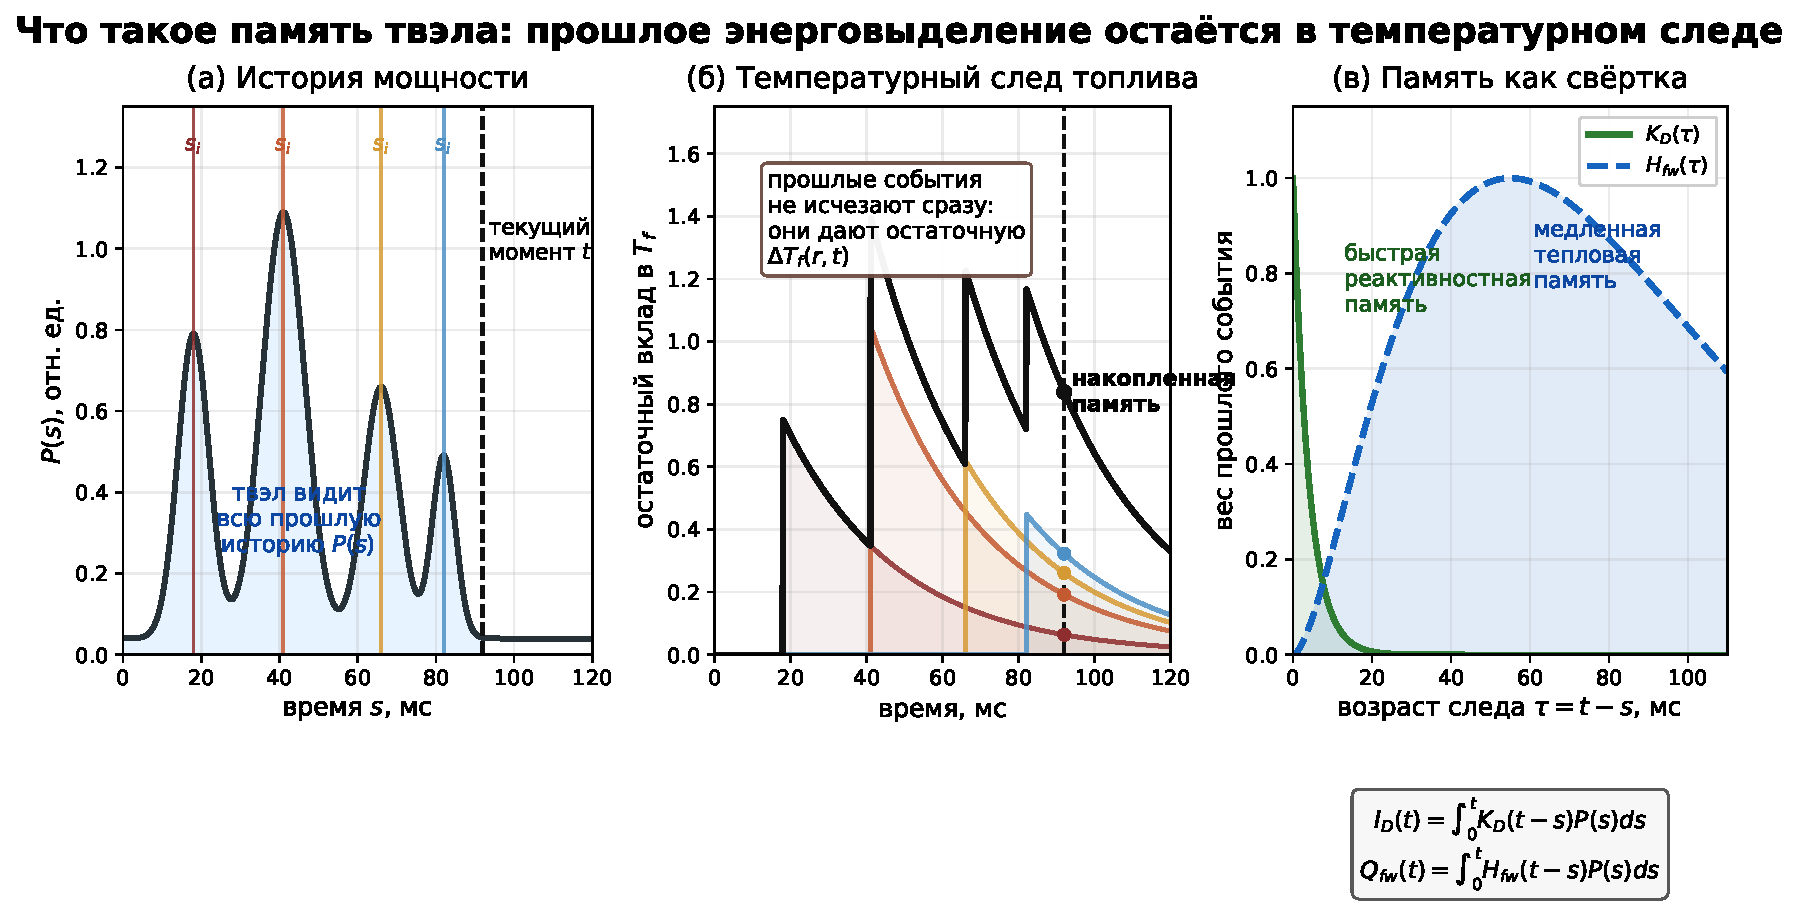
\includegraphics[width=\textwidth]{figures/fig0_fuel_memory_concept.pdf}
\caption{Физический смысл памяти твэла: история мощности создаёт остаточный температурный след, который затем взвешивается двумя ядрами памяти \(K_D\) и \(H_{fw}\).}
\label{fig:fuelMemoryConcept}
\end{figure}

\section{Теоретическая модель: твэл как спектрально-тепловой элемент памяти}

\subsection{Физическая постановка и иерархия описания}

В обычной инженерной записи топливная обратная связь часто сводится к одной строке:
\[
\rho_D=\alpha_D\Delta T_f.
\]
Такая запись верна как локальная линеаризация около стационарного состояния, но она скрывает главный механизм переходного процесса. В импульсном режиме температура топлива не является заданным параметром. Она является следом уже произошедшего энерговыделения. Поэтому причинная цепочка имеет вид
\[
\boxed{
P(s)
\rightarrow
q'''(\mathbf r,s)
\rightarrow
T_f(\mathbf r,t)
\rightarrow
\sigma_a(E,T_f)
\rightarrow
\rho_D(t)
\rightarrow
P(t).
}
\]
Здесь причина и следствие разведены во времени: мощность в прошлом создаёт тепловой след, а этот след в настоящем меняет вероятность выживания нейтронов.

Центральная идея работы состоит в том, что твэл следует рассматривать не как пассивный источник тепла для теплоносителя, а как элемент памяти. Один и тот же температурный след имеет два выхода. Первый выход является реактивностным: нагретое топливо уширяет резонансы поглощения и создаёт отрицательную доплеровскую реактивность. Второй выход является тепловым: часть энергии с запаздыванием проходит через топливо, зазор, оболочку и поверхность теплообмена к воде. В этом смысле твэл действует как двухканальный причинный оператор:
\[
P(t)
\longrightarrow
\begin{cases}
I_D(t)=K_D*P, & \text{доплеровская реактивностная память},\\[3pt]
Q_{fw}(t)=H_{fw}*P, & \text{задержанный тепловой поток к воде}.
\end{cases}
\]
Физическая основа первого канала стандартна: рост температуры топлива приводит к уширению резонансов поглощения, особенно в тяжёлых изотопах, и тем самым обычно увеличивает резонансный захват нейтронов \cite{NRCFeedback2012,DOEGeneralTechnicalBase2013}. Новизна данной постановки не в самом существовании доплеровского коэффициента, а в замене статического коэффициента геометрически определённой функцией памяти.

Для дальнейшего изложения удобно разделить переменные на три уровня. Быстрый уровень содержит нейтронную мощность \(P(t)\), группы предшественников \(C_i(t)\), фазово-пространственное распределение нейтронов \(f_n(\mathbf r,\mathbf p,t)\) и температурное поле топлива \(T_f(\mathbf r,t)\). Средний уровень содержит тепловой выход к поверхности твэла и теплоносителю. Медленный уровень содержит плотность теплоносителя, паросодержание, давление и возможное механическое изменение геометрии. В данной работе медленный уровень сохраняется как функционал
\[
\rho_{\mathrm{slow}}(t)
=
\mathcal R_{\mathrm{slow}}
[T_c,\rho_c,\alpha_v,p,\mathbf q],
\]
но не является первичным объяснением импульса. Главный объект теории --- быстрый спектрально-тепловой контур
\[
P\rightarrow T_f\rightarrow \sigma_a(E,T_f)\rightarrow I_D\rightarrow \rho_D.
\]

\subsection{От траектории нейтрона к локальному энерговыделению}

Микроскопически нейтрон внутри топлива не отдаёт энергию непрерывно. Между столкновениями его движение можно записать как
\[
\frac{d\mathbf r}{dt}=\frac{\mathbf p}{m_n},
\qquad
\frac{d\mathbf p}{dt}\approx0,
\]
а взаимодействие с веществом происходит как скачок состояния или как исчезновение нейтрона из данной траектории при поглощении или делении. Для событий
\[
j\in\{s,\gamma,f\},
\]
где \(s\) обозначает рассеяние, \(\gamma\) --- радиационный захват, а \(f\) --- деление, интенсивность события равна
\[
\lambda_j(\mathbf r,\mathbf p,t)
=
v(p)\Sigma_j(E,T_f(\mathbf r,t)).
\]
За малое время \(dt\)
\[
d\mathbb P_j=\lambda_j\,dt.
\]
Эта запись важна методически: температура топлива влияет не на ``теплоту'' как таковую, а на вероятности ядерных событий. Когда растёт \(T_f\), меняются температурно-зависимые макроскопические сечения, прежде всего резонансная часть поглощения
\[
\lambda_{\mathrm{res}}
=
v\Sigma_{a,\mathrm{res}}(E,T_f).
\]
Следовательно, нагрев топлива меняет судьбу последующих нейтронов: часть из них поглощается в резонансной области до того, как сможет поддержать дальнейшую цепочку делений.

Локальная плотность энерговыделения получается усреднением по ансамблю таких траекторий:
\[
q'''(\mathbf r,t)
=
\int
f_n(\mathbf r,\mathbf p,t)v(p)
\left[
\Sigma_f(E,T_f)Q_f^{\mathrm{dep}}
+
\Sigma_\gamma(E,T_f)Q_\gamma^{\mathrm{dep}}
+
\Sigma_s(E,T_f)\langle\Delta E_s\rangle
\right]d^3p.
\]
В этой формуле \(Q_f^{\mathrm{dep}}\) --- локально депонируемая часть энергии деления, \(Q_\gamma^{\mathrm{dep}}\) --- энергия, депонируемая после радиационного захвата, а \(\langle\Delta E_s\rangle\) --- средняя передача энергии при рассеянии. Нейтрон в такой картине является не главным носителем энергии, а триггером ядерного события: большая доля энергии деления быстро оказывается в кинетической энергии осколков и затем в тепле топлива \cite{DOEGeneralTechnicalBase2013}.

Переход к reduced-модели требует отделить форму источника от его амплитуды. Если во время рассматриваемого импульса пространственно-энергетическая форма нейтронного поля меняется слабее, чем его амплитуда, можно записать
\[
f_n(\mathbf r,\mathbf p,t)\approx A(t)f_0(\mathbf r,\mathbf p),
\]
а значит
\[
q'''(\mathbf r,t)=a(\mathbf r)P(t),
\qquad
\int_{\Omega_f}a(\mathbf r)dV=1.
\]
Здесь \(\Omega_f\) --- область топлива, \(P(t)\) --- полная мощность, а \(a(\mathbf r)\) имеет размерность обратного объёма. Это не утверждение о равномерном нагреве. Напротив, вся геометрическая информация о месте рождения теплового следа сохраняется в функции \(a(\mathbf r)\).

\subsection{Доплеровское уширение как импульсная статистика ядер}

Доплеровский эффект в топливе лучше всего понимать не как эмпирическую температурную поправку к сечению, а как усреднение микроскопического резонанса по импульсам ядер. Нейтрон с импульсом \(\mathbf p\) взаимодействует не с неподвижным ядром, а с ядром, имеющим тепловую скорость \(\mathbf u_A\). Относительная энергия столкновения равна
\[
E_{\mathrm{rel}}
=
\frac{1}{2}\mu|\mathbf v_n-\mathbf u_A|^2,
\]
где \(\mu\) --- приведённая масса. Если скорости ядер распределены по Максвеллу,
\[
M(\mathbf u_A;T_f)
=
\left(\frac{M_A}{2\pi k_BT_f}\right)^{3/2}
\exp\left(-\frac{M_Au_A^2}{2k_BT_f}\right),
\]
то температурно-уширенное сечение можно формально записать как
\[
\sigma_a^D(E,T_f)
=
\int\sigma_a^{(0)}(E_{\mathrm{rel}})
M(\mathbf u_A;T_f)d^3u_A.
\]
При увеличении \(T_f\) распределение импульсов ядер расширяется, узкий резонанс ``размазывается'' по энергии, а эффективный резонансный захват для проходящего спектра нейтронов возрастает. Поэтому физическая цепочка имеет вид
\[
T_f\uparrow
\Rightarrow
M(\mathbf u_A;T_f)\ \text{шире}
\Rightarrow
\sigma_a(E,T_f)\ \text{шире в резонансах}
\Rightarrow
\Sigma_{a,\mathrm{res}}\uparrow
\Rightarrow
\rho_D<0.
\]
В вычислительной перспективе этот уровень может быть проверен независимыми расчётами температурно-зависимых сечений; например, документация OpenMC описывает windowed multipole representation, позволяющее выполнять Doppler broadening к произвольной температуре \cite{OpenMCCrossSections}.

\begin{figure}[H]
\centering
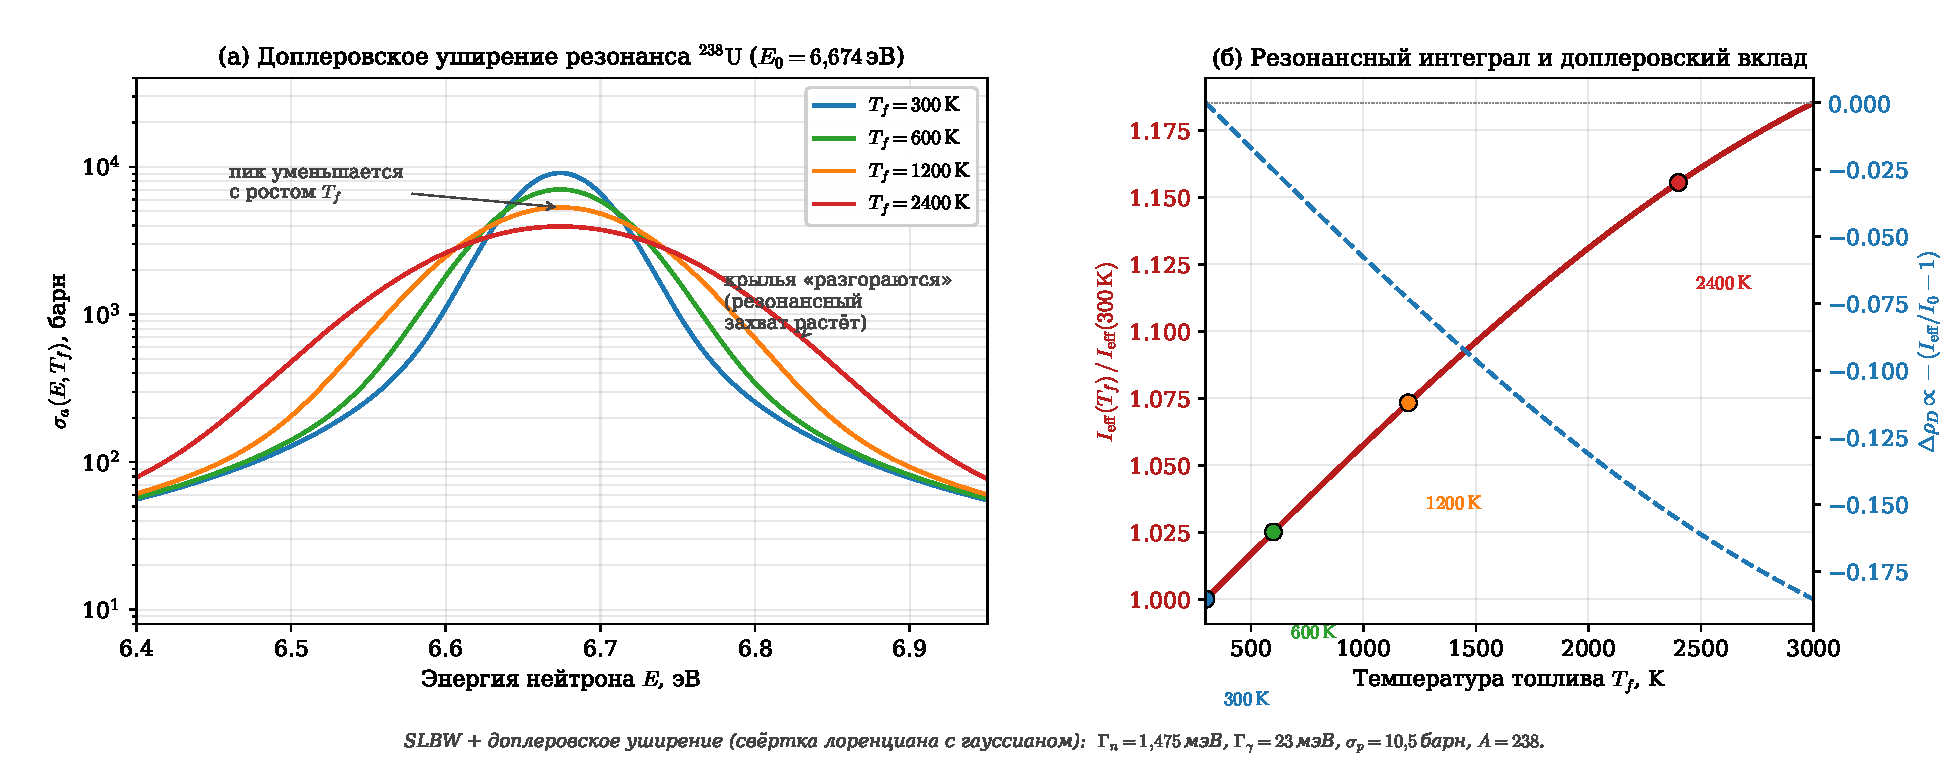
\includegraphics[width=\textwidth]{figures/fig2_doppler.pdf}
\caption{Иллюстративное доплеровское уширение резонанса \(^{238}\mathrm{U}\). В теории памяти важно не только изменение формы резонанса, но и то, что это изменение возникает из температурного следа, созданного предыдущей историей мощности.}
\label{fig:doppler}
\end{figure}

\subsection{Тепловой след в геометрии топлива}

После ядерных событий энергия становится источником для теплопроводности. В линеаризованной постановке относительно исходного состояния \(T_{f0}\) температурное возмущение удовлетворяет уравнению
\[
\rho_f c_{p,f}\frac{\partial \Delta T_f}{\partial t}
=
\nabla\cdot\left(\lambda_f\nabla\Delta T_f\right)
+
q'''(\mathbf r,t),
\qquad
\mathbf r\in\Omega_f.
\]
Граничные условия могут содержать зазор, оболочку и теплообмен с теплоносителем; на теоретическом уровне они входят в оператор теплопроводности. Пусть \(G_T(\mathbf r,\mathbf r',\tau)\) --- причинная функция Грина этой задачи. Тогда
\[
\Delta T_f(\mathbf r,t)
=
\int_0^t\int_{\Omega_f}
G_T(\mathbf r,\mathbf r',t-s)a(\mathbf r')P(s)dV'ds.
\]
Эта формула является первым местом, где геометрия твэла входит строго, а не иллюстративно. Геометрия задаёт, куда был помещён источник \(a(\mathbf r')\), как тепло распространилось через \(G_T\), и какие области топлива остались нагретыми к моменту \(t\).

Важно, что \(\Delta T_f(\mathbf r,t)\) не обязана следовать за \(P(t)\) мгновенно. Даже если мощность имеет узкий пик, температурное поле является интегралом по прошлому. Поэтому правильный объект теории --- не текущая средняя температура, а пространственно-временной тепловой след:
\[
\mathcal T_f(t)=\{\Delta T_f(\mathbf r,t):\mathbf r\in\Omega_f\}.
\]
Реактивностный и тепловой выходы являются двумя различными функционалами от одного и того же следа.

\subsection{Реактивностный функционал и поле доплеровской важности}

Реактивность можно рассматривать как функционал температурного поля топлива:
\[
\rho=\rho[T_f(\mathbf r)].
\]
При малом возмущении около базового состояния
\[
\delta\rho
=
\int_{\Omega_f}
\frac{\delta\rho}{\delta T_f(\mathbf r)}
\Delta T_f(\mathbf r,t)dV.
\]
Для отрицательной топливной обратной связи удобно ввести положительное поле доплеровской важности
\[
D_D(\mathbf r)
=
-\frac{\delta\rho}{\delta T_f(\mathbf r)}>0.
\]
Тогда
\[
\rho_D(t)
=
-\int_{\Omega_f}D_D(\mathbf r)\Delta T_f(\mathbf r,t)dV.
\]
Поле \(D_D(\mathbf r)\) отвечает на простой физический вопрос: насколько нагрев именно этой части топлива уменьшает реактивность всей системы? Поэтому два одинаковых по энергии тепловых события могут иметь разный реактивностный вес, если они произошли в разных местах или в разных спектральных условиях.

Подставляя решение теплопроводности в реактивностный функционал, получаем
\[
\rho_D(t)
=
-\int_0^tK_D(t-s)P(s)ds,
\]
где
\[
\boxed{
K_D(\tau)
=
\int_{\Omega_f}\int_{\Omega_f}
D_D(\mathbf r)
G_T(\mathbf r,\mathbf r',\tau)
a(\mathbf r')dV'dV.
}
\]
Это главный математический объект теоретической части. Он объединяет в одной формуле нейтронную форму энерговыделения, теплопроводность, геометрию топлива и реактивностную важность нагрева. Если \(P\) измеряется в ваттах, а \(\rho\) безразмерна, то \(K_D\) имеет размерность \(1/\mathrm{J}\); при записи реактивности в pcm --- \(\mathrm{pcm}/\mathrm{J}\).

Удобно также ввести накопленную доплеровскую память
\[
I_D(t)=\int_0^tK_D(t-s)P(s)ds,
\qquad
\rho_D(t)=-I_D(t).
\]
Тогда физический смысл модели становится предельно ясным:
\[
P(t)\uparrow
\Rightarrow
q'''\uparrow
\Rightarrow
T_f\uparrow
\Rightarrow
I_D\uparrow
\Rightarrow
\rho_{\mathrm{eff}}\downarrow
\Rightarrow
P(t)\downarrow.
\]
Импульс мощности записывает в твэле тепловую память, а эта память становится отрицательной реактивностью.

\subsection{Тепловой канал к воде}

Тот же температурный след создаёт второй выход --- тепловой поток через поверхность теплообмена. Пусть \(\Gamma_w\) обозначает эффективную поверхность передачи тепла к водному каналу. В простейшей записи
\[
Q_{fw}(t)
=
\int_{\Gamma_w}
\left[-\lambda_f\nabla\Delta T_f(\mathbf r,t)\cdot\mathbf n\right]dS,
\]
или, если оболочка и зазор уже включены в эффективный граничный оператор, \(Q_{fw}\) следует понимать как соответствующий линейный тепловой функционал. Обозначим этот граничный функционал через \(\mathcal B_w\). Тогда
\[
Q_{fw}(t)=\mathcal B_w[\Delta T_f(\cdot,t)].
\]
После подстановки функции Грина получается вторая свёртка:
\[
Q_{fw}(t)
=
\int_0^tH_{fw}(t-s)P(s)ds,
\]
\[
\boxed{
H_{fw}(\tau)
=
\mathcal B_w\left[
\int_{\Omega_f}G_T(\cdot,\mathbf r',\tau)a(\mathbf r')dV'
\right].
}
\]
Если записывать граничный поток явно через градиент температуры, то
\[
H_{fw}(\tau)=
\int_{\Gamma_w}\int_{\Omega_f}
\left[-\lambda_f\nabla_{\mathbf r}G_T(\mathbf r,\mathbf r',\tau)\cdot\mathbf n\right]
a(\mathbf r')dV'dS.
\]
Таким образом, \(K_D\) и \(H_{fw}\) являются не двумя независимыми гипотезами, а двумя проекциями одного теплового следа. Первое ядро взвешивает объёмный нагрев по реактивностной важности, второе --- по способности этого нагрева выйти через поверхность теплообмена.

\begin{figure}[H]
\centering
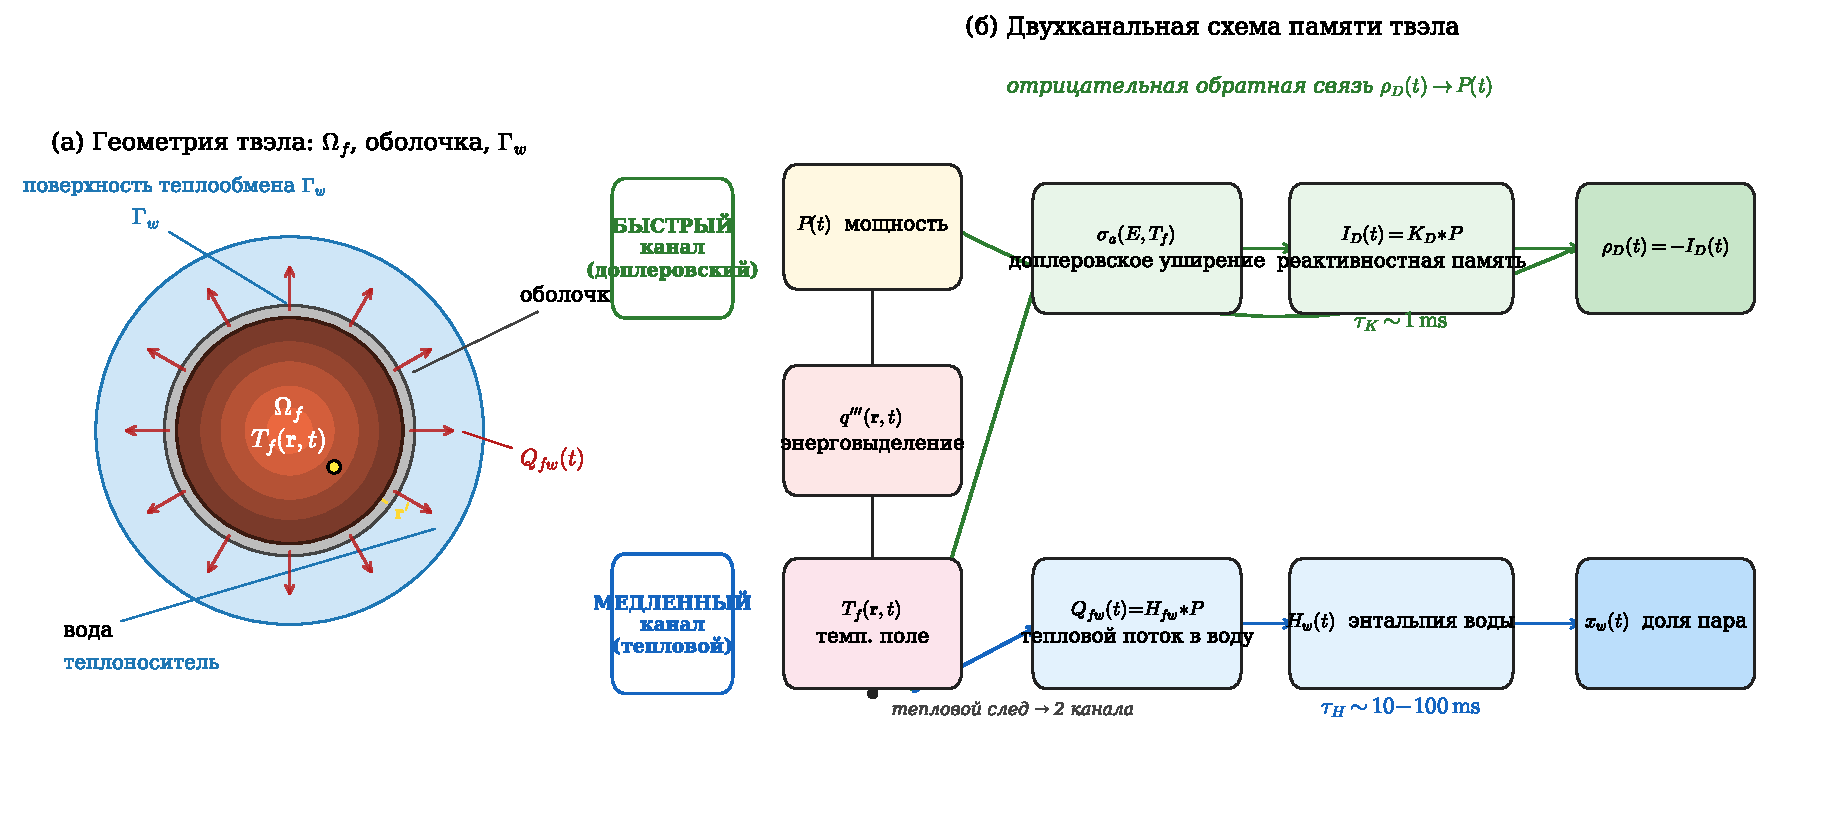
\includegraphics[width=\textwidth]{figures/fig1_twoChannel.pdf}
\caption{Двухканальная схема памяти твэла: история мощности создаёт один температурный след, но два разных наблюдаемых выхода --- реактивностный \(I_D=K_D*P\) и тепловой \(Q_{fw}=H_{fw}*P\).}
\label{fig:twoChannel}
\end{figure}

\subsection{Причинность, знаки и энергетические ограничения}

Обе функции памяти должны быть причинными:
\[
K_D(\tau)=0,
\qquad
H_{fw}(\tau)=0,
\qquad
\tau<0.
\]
При выбранной записи \(\rho_D=-I_D\) физически ожидаемый доплеровский kernel неотрицателен:
\[
K_D(\tau)\ge0.
\]
Это означает, что положительный импульс мощности создаёт положительную память \(I_D\), а она входит в реактивность со знаком минус. Для теплового канала в идеальной линейной модели без артефактов baseline-subtraction также ожидается
\[
H_{fw}(\tau)\ge0.
\]
Интеграл теплового ядра имеет смысл доли энергии, которая в пределе бесконечного времени выходит через выбранный канал:
\[
\eta_w(\infty)
=
\int_0^\infty H_{fw}(\tau)d\tau.
\]
Если \(Q_{fw}\) включает только поток из топлива в воду, то \(\eta_w(\infty)\le1\), поскольку часть энергии может оставаться в других элементах баланса или уходить через другие каналы. На конечном окне наблюдения корректно писать
\[
\mathcal W(t_{\mathrm{obs}})
=
\frac{\int_0^{t_{\mathrm{obs}}}Q_{fw}(t)dt}{\int_0^{t_{\mathrm{obs}}}P(t)dt},
\]
и не отождествлять эту величину с полной асимптотической долей энергии.

\begin{table}[H]
\centering
\caption{Основные величины теоретической модели и их размерности.}
\label{tab:units}
\begin{tabular}{|>{\centering\arraybackslash}p{3.2cm}|p{7.0cm}|>{\centering\arraybackslash}p{3.0cm}|}
\hline
Величина & Смысл & Единицы\\
\hline
\(P(t)\) & мощность или baseline-subtracted excess power & W\\
\(a(\mathbf r)\) & нормированная форма энерговыделения & \(\mathrm{m^{-3}}\)\\
\(G_T\) & тепловая функция Грина топлива и граничного слоя & K/J\\
\(D_D(\mathbf r)\) & локальная доплеровская важность нагрева & \(1/(\mathrm{K\,m^3})\) или pcm/(K m\(^3\))\\
\(K_D(t)\) & реактивностное ядро памяти & \(1/\mathrm{J}\) или pcm/J\\
\(I_D(t)\) & накопленная доплеровская память & 1 или pcm\\
\(H_{fw}(t)\) & тепловое ядро выхода к воде & \(\mathrm{s^{-1}}\)\\
\(Q_{fw}(t)\) & тепловой поток в водный канал & W\\
\(\mathcal D_{\mathrm{ext}},\mathcal W\) & критерии режима & безразмерные\\
\hline
\end{tabular}
\end{table}

\subsection{Нелинейная кинетика с памятью}

На уровне точечной кинетики с группами запаздывающих нейтронов \cite{DuderstadtHamilton1976}
\[
\frac{dP}{dt}
=
\frac{\rho_{\mathrm{eff}}(t)-\beta}{\Lambda}P
+
\sum_i\lambda_iC_i+S(t),
\]
\[
\frac{dC_i}{dt}
=
\frac{\beta_i}{\Lambda}P-\lambda_iC_i.
\]
В предлагаемой модели эффективная реактивность имеет вид
\[
\rho_{\mathrm{eff}}(t)
=
\rho_0+\rho_{\mathrm{ext}}(t)-I_D(t)+\rho_{\mathrm{slow}}(t),
\]
\[
I_D(t)=\int_0^tK_D(t-s)P(s)ds.
\]
Здесь \(\rho_{\mathrm{ext}}\) обозначает внешнюю вставку реактивности, если она присутствует, а \(\rho_{\mathrm{slow}}\) собирает медленные теплогидравлические и механические обратные связи. В отличие от записи \(\rho_D=\alpha_D\Delta T_f\), эта система не является марковской по \(P(t)\): будущая динамика зависит от тепловой памяти, накопленной всей предыдущей историей мощности.

Условие максимума мощности получается из \(dP/dt=0\):
\[
\frac{\rho_{\mathrm{eff}}(t_{\max})-\beta}{\Lambda}P(t_{\max})
+
\sum_i\lambda_iC_i(t_{\max})+S(t_{\max})=0.
\]
Поэтому пик мощности не обязан совпадать с условием \(\rho_{\mathrm{eff}}=0\). Запаздывающие нейтроны и внешний источник смещают точку максимума. Тем не менее в физическом смысле пик возникает тогда, когда накопленная отрицательная память \(I_D\) становится сравнимой с положительным реактивностным запасом, действующим на рассматриваемом интервале.

Теоретический критерий самогашения можно записать как
\[
\boxed{
I_D(t_*)
\gtrsim
\rho_0+
\sup_{0<s<t_*}\rho_{\mathrm{ext}}^+(s)
+
\sup_{0<s<t_*}\rho_{\mathrm{slow}}^+(s).
}
\]
Он выражает энергетически простую мысль: импульс самогасится, если успевает создать такую доплеровскую тень, которая перекрывает положительный реактивностный вклад. Но одной амплитуды недостаточно. Нужно также временное условие
\[
\tau_K\lesssim\tau_{\mathrm{growth}},
\]
где
\[
\tau_K
=
\frac{\int_0^\infty \tau K_D(\tau)d\tau}{\int_0^\infty K_D(\tau)d\tau}
\]
--- характерное время доплеровского отклика, а \(\tau_{\mathrm{growth}}\) --- время роста мощности. Если \(\tau_K\ll\tau_{\mathrm{growth}}\), обратная связь почти мгновенно ограничивает рост. Если \(\tau_K\sim\tau_{\mathrm{growth}}\), возникает перерегулирование. Если \(\tau_K\gg\tau_{\mathrm{growth}}\), доплеровская память приходит слишком поздно, и режим остаётся внешне вынужденным.

\subsection{Реализация памяти через конечное число мод}

Для расчётной reduced-модели свёртки удобно аппроксимировать суммами экспонент:
\[
K_D(t)=\sum_jA_je^{-t/\tau_j},
\qquad
H_{fw}(t)=\sum_jB_je^{-t/\theta_j}.
\]
Тогда интегральная память заменяется дополнительными переменными состояния:
\[
\dot z_j=P-\frac{z_j}{\tau_j},
\qquad
I_D=\sum_jA_jz_j,
\]
\[
\dot y_j=P-\frac{y_j}{\theta_j},
\qquad
Q_{fw}=\sum_jB_jy_j.
\]
Такая форма полезна по двум причинам. Во-первых, она превращает задачу с памятью в обычную систему ОДУ, пригодную для построения карт режимов. Во-вторых, параметры \(A_j,\tau_j,B_j,\theta_j\) имеют физическую интерпретацию: быстрые моды соответствуют локальному нагреву топлива и ранней доплеровской реакции, медленные --- тепловой инерции и выходу энергии через оболочку и теплоноситель. В этой логике OpenFOAM, MOOSE и GeN-Foam выступают не заменой теории, а источниками или проверкой параметров теплового и мультифизического слоя \cite{MOOSEHeatTransfer,OpenFOAMSolvers,GeNFoam2015}.

\begin{figure}[H]
\centering
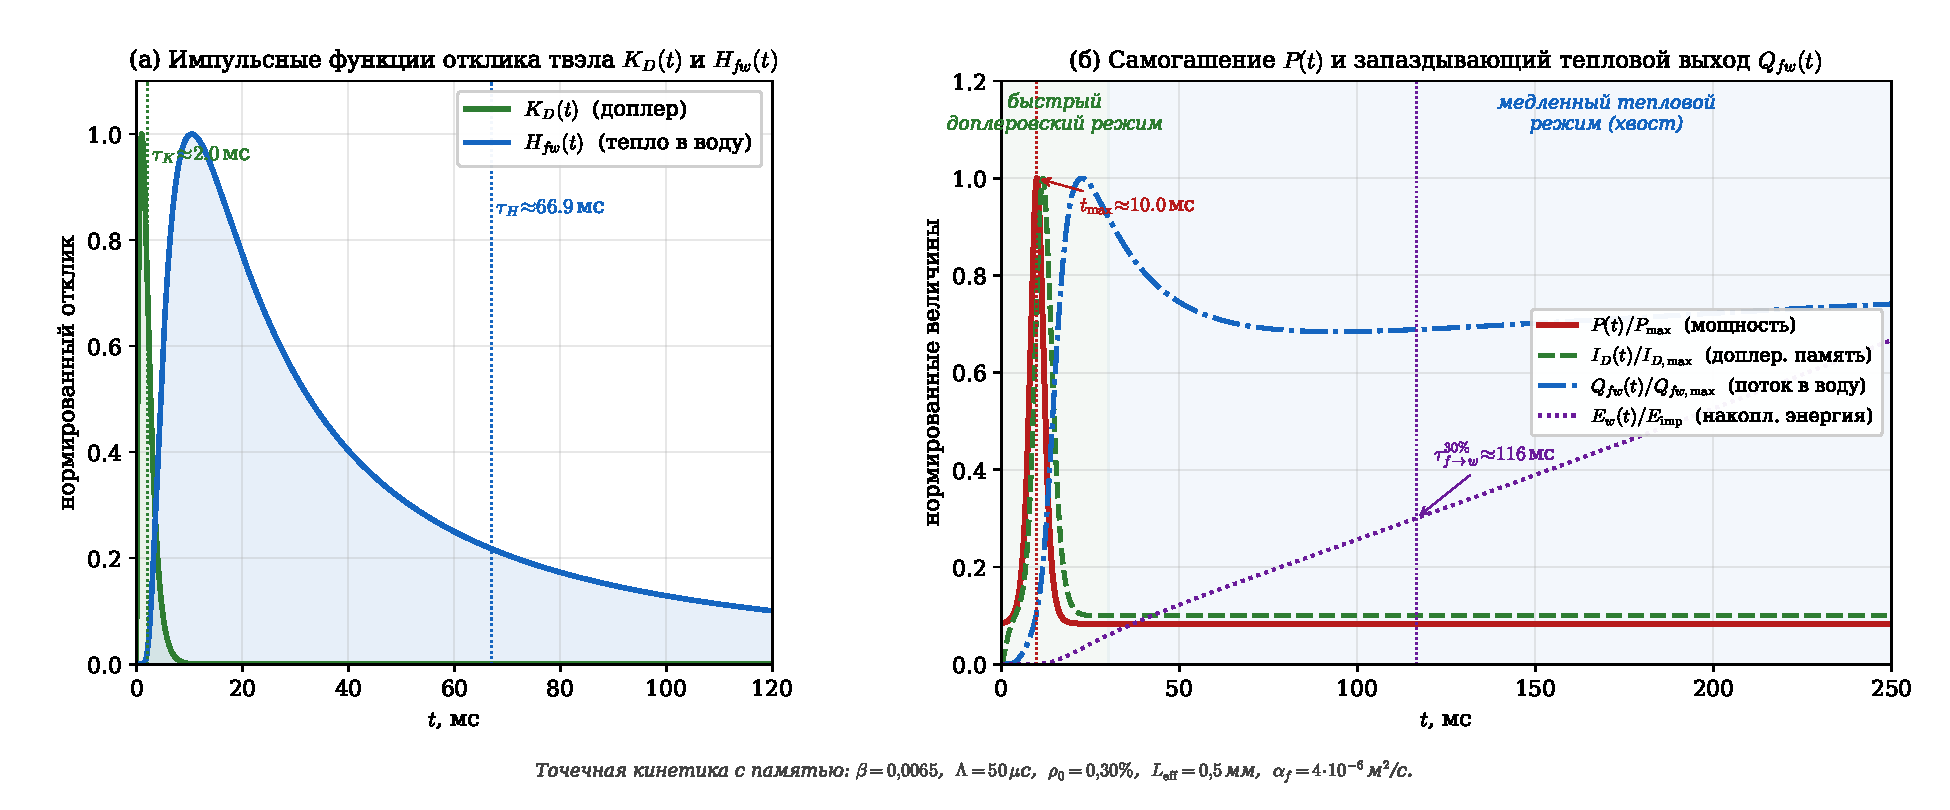
\includegraphics[width=\textwidth]{figures/fig3_dynamics.pdf}
\caption{Иллюстративный reduced-model расчёт целевого режима: быстрый рост \(I_D\) ограничивает мощность раньше, чем значительная часть энергии выходит в водный канал. Этот рисунок задаёт физическую цель модели, а не параметры конкретного GeN-Foam benchmark.}
\label{fig:dynamics}
\end{figure}

\subsection{Классификация режимов}

Модель памяти позволяет различать несколько физически разных режимов, которые в обычной записи могут выглядеть похожими.

Первый режим --- доплеровски самогасящийся импульс. Для него выполняются одновременно амплитудное условие \(I_D\) сравнимо с положительной реактивностью и временное условие \(\tau_K\lesssim\tau_{\mathrm{growth}}\). Мощность имеет один выраженный максимум, созданный не выключением внешнего воздействия, а накопленной топливной памятью.

Второй режим --- импульс с перерегулированием. Здесь \(K_D\) достаточно силён, но не мгновенен. Мощность успевает превысить квазистационарный уровень, после чего подавляется запаздывающей отрицательной реактивностью.

Третий режим --- теплогидравлически модифицированный импульс. В этом случае \(\rho_{\mathrm{slow}}\) становится сравнимым с \(I_D\), и вода, плотность, паросодержание или механика меняют хвост импульса. Главный пик всё ещё может быть доплеровским, но последующая эволюция уже не определяется только топливом.

Четвёртый режим --- слабосвязанный внешне вынужденный transient. Для него
\[
\mathcal D_{\mathrm{ext}}
=
\frac{I_D^{\max}}{\rho_{\mathrm{ext}}^{\max}}
\ll1.
\]
В таком режиме спад мощности определяется главным образом формой внешней вставки или внешнего источника, а не самогашением топлива. Именно к этому классу, как будет показано ниже, относится текущий GeN-Foam benchmark.

Пятый режим --- потеря применимости reduced-модели. Она наступает, если нарушаются приближения
\[
f_n(\mathbf r,\mathbf p,t)\approx A(t)f_0(\mathbf r,\mathbf p),
\qquad
q'''(\mathbf r,t)\approx a(\mathbf r)P(t),
\]
если спектр нейтронов перестраивается на масштабе самого импульса, либо если двухфазная теплогидравлика становится не медленной поправкой, а главным динамическим каналом. Эта граница применимости является частью результата: модель должна не только объяснять целевой режим, но и показывать, когда данный расчёт к нему не относится.

\section{Масштабы теплового отклика и связь с водой}

\subsection{Почему вода не видит нейтронный импульс мгновенно}

Тепловой канал нельзя оценивать по длительности нейтронного пика. После локального энерговыделения тепло распространяется диффузионно, и характерная глубина проникновения за время \(t\) равна
\[
\ell_T(t)\sim\sqrt{\alpha_f t},
\qquad
\alpha_f=\frac{\lambda_f}{\rho_fc_{p,f}}.
\]
Для типичного порядка \(\alpha_f\sim10^{-6}\,\mathrm{m^2/s}\) за \(1\,\mathrm{ms}\) тепловое возмущение проходит только десятки микрон. Следовательно, доплеровский канал может включаться на раннем масштабе, потому что он чувствует объёмный нагрев топлива, тогда как водный канал ждёт, пока энергия дойдёт до поверхности теплообмена.

Более строго тепловой выход можно представить как сумму собственных тепловых мод оператора теплопроводности:
\[
G_T(\mathbf r,\mathbf r',t)
=
\sum_n\phi_n(\mathbf r)\phi_n^*(\mathbf r')e^{-t/\tau_n}.
\]
Тогда оба ядра имеют модовую структуру:
\[
K_D(t)=\sum_n k_ne^{-t/\tau_n},
\qquad
H_{fw}(t)=\sum_n h_ne^{-t/\tau_n},
\]
но коэффициенты \(k_n\) и \(h_n\) различны. Реактивностный канал взвешивает моды объёмным функционалом \(D_D\), а водный канал --- граничным тепловым функционалом. Поэтому у двух каналов могут быть разные эффективные времена даже при одном и том же уравнении теплопроводности.

\subsection{Оценка времени выхода энергии к поверхности}

Грубая диффузионная оценка времени выхода тепла к поверхности имеет вид
\[
\tau_{f\to w}
\sim
c_\eta\frac{L_{\mathrm{eff}}^2}{\alpha_f}
+
\frac{\delta_{\mathrm{barrier}}^2}{\alpha_b}
+\tau_{\mathrm{int}}.
\]
Здесь \(L_{\mathrm{eff}}\) --- эффективное расстояние от области энерговыделения до поверхности теплообмена, \(\delta_{\mathrm{barrier}}\) --- толщина теплового барьера, \(\alpha_b\) --- его температуропроводность, \(\tau_{\mathrm{int}}\) --- дополнительная интерфейсная или sub-scale инерция, а \(c_\eta\) зависит от выбранной доли вышедшей энергии. Эта формула не претендует на универсальную константу. Она показывает масштабный закон: тепловая задержка квадратично растёт с расстоянием и линейно уменьшается с температуропроводностью.

Из этого следует важное методическое правило. Миллисекундный нейтронный импульс и секундный хвост \(H_{fw}\) не противоречат друг другу. Первый относится к цепной реакции и объёмному нагреву топлива; второй --- к прохождению энергии через тепловые барьеры и к конкретной sub-scale модели теплообмена.

\subsection{Связь теории с GeN-Foam постановкой}

В рассматриваемом GeN-Foam case тепловой канал следует понимать как эффективное ядро конкретной мультифизической постановки. GeN-Foam является OpenFOAM-based инструментом для стационарного и переходного анализа ядерных реакторов \cite{GeNFoam2015}; более новая линия foamForNuclear развивает unified OpenFOAM multiphysics architecture для ядерных приложений \cite{foamForNuclear2026}. Поэтому величина \(H_{fw}\), восстановленная из такого расчёта, не обязана совпадать с простой аналитической оценкой чистой теплопроводности в цилиндре. Она включает то, как конкретная модель представляет топливо, оболочку, интерфейс и теплообмен с теплоносителем.

Практический вывод состоит в следующем. Если за окно наблюдения \(t_{\mathrm{obs}}\) в воду уходит доля \(\mathcal W(t_{\mathrm{obs}})\), то оставшаяся excess-энергия не исчезает. Она остаётся в тепловой инерции топлива, оболочки, теплоносителя или в других членах энергетического баланса. Поэтому в численной части нужно различать три утверждения:
\[
\begin{gathered}
\text{энергия выделилась в топливе},\\
\text{энергия создала доплеровскую память},\\
\text{энергия дошла до водного канала}.
\end{gathered}
\]
Именно это разделение делает двухканальную модель полезной: она не смешивает реактивностную роль раннего нагрева топлива с поздним тепловым выходом к воде.


\section{GeN-Foam и роль benchmark в работе}

GeN-Foam -- это открытый мультифизический расчётный код на базе OpenFOAM, предназначенный для моделирования переходных процессов в ядерных реакторах \cite{GeNFoam2015,foamForNuclear2026}. Его важная особенность состоит в том, что нейтроника, теплогидравлика и теплообмен в твёрдых структурах решаются в одной связанной постановке. В зависимости от выбранной модели GeN-Foam может использовать точечную кинетику или пространственную нейтронику, однофазную или двухфазную теплогидравлику, а также sub-scale модели твэлов и твёрдых конструкций.

В данной работе используется связка моделей \texttt{pointKinetics}, \texttt{onePhase} и \texttt{nuclearFuelPin}. Точечная кинетика задаёт динамику мощности и реактивности, однофазная теплогидравлика описывает теплоноситель, а модель \texttt{nuclearFuelPin} рассчитывает эффективный одномерный теплообмен внутри твэла и передаёт тепловой поток в жидкостную область. Поэтому GeN-Foam здесь не является инструментом прямого восстановления пространственного поля \(D_D(\mathbf r)\). Его роль более узкая: дать самосогласованные временные ряды мощности, температур, топливной обратной связи и теплового потока к воде в конкретной мультифизической постановке.

\begin{figure}[H]
    \centering
    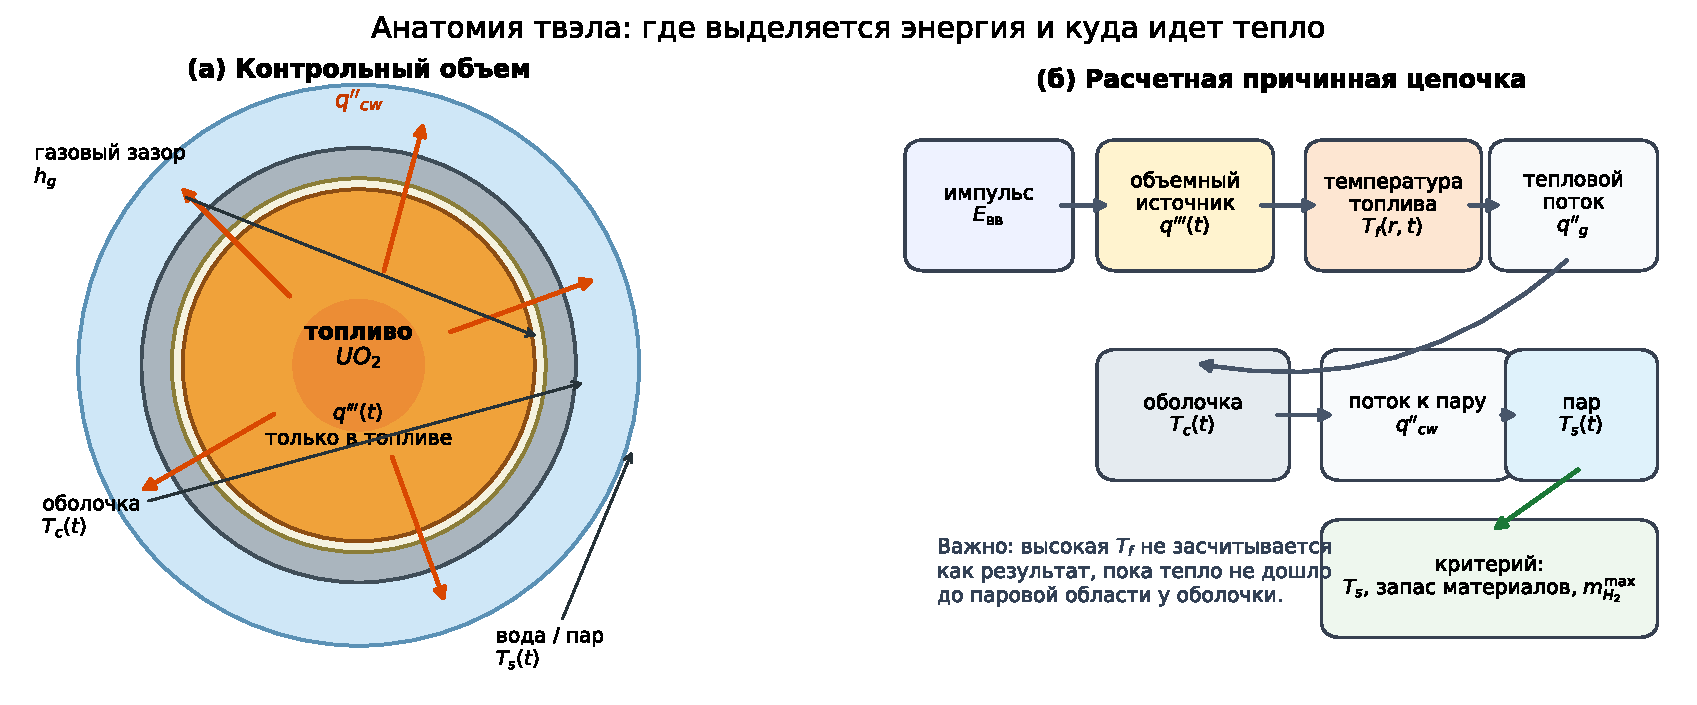
\includegraphics[width=\textwidth]{figures/fig7_fuel_pin_anatomy.pdf}
    \caption{Схема физического процесса в твэле, используемая для интерпретации GeN-Foam benchmark. Энерговыделение \(q'''(r)\) возникает в топливе \(UO_2\), создаёт радиальный температурный профиль \(T_f(r,t)\), проходит через газовый зазор и циркониевую оболочку, а затем выходит в воду как \(Q_{fw}(t)\). В этой же топливной области формируется доплеровский реактивностный след \(I_D=K_D*P\).}
    \label{fig:fuelPinAnatomy}
\end{figure}

Рис.~\ref{fig:fuelPinAnatomy} показывает, почему в работе разделяются два выхода одного и того же импульса мощности. Доплеровская реактивность определяется объёмным нагревом топлива и может появляться раньше, чем тепло достигнет поверхности теплообмена. Водный канал, наоборот, видит энергию только после прохождения через топливо, зазор, оболочку и интерфейс с теплоносителем; поэтому \(H_{fw}\) имеет более длинную память.

Под benchmark в этой работе понимается не экспериментальный эталон, а фиксированный воспроизводимый расчётный сценарий. Он задаёт начальное состояние, внешнюю вставку реактивности, набор физических моделей, сетку, параметры твэла, способ вывода полей и процедуру постобработки. Такой сценарий нужен для того, чтобы не обсуждать модель памяти только на уровне формул, а проверить, какие диагностические величины можно извлечь из реального coupled transient:
\[
P(t),\quad
\Delta\rho_f(t),\quad
T_f(t),\quad
Q_{fw}(t),\quad
E_w(t).
\]
Именно из этих временных рядов затем строятся baseline-subtracted сигналы, критерии \(\mathcal D_{\mathrm{ext}}\) и \(\mathcal W(t_{\mathrm{obs}})\), а также попытка идентификации ядер \(K_D\) и \(H_{fw}\).

Benchmark нужен в работе по трём причинам. Во-первых, он проверяет диагностическую процедуру: можно ли по расчётным данным отделить собственный отклик на импульс от фонового дрейфа. Во-вторых, он показывает, какой из двух каналов памяти реально виден в выбранной постановке. В-третьих, он служит контрпримером к целевому Doppler-active режиму: если \(\mathcal D_{\mathrm{ext}}\ll1\), то спад мощности нельзя честно объяснять доплеровским самогашением, даже если в модели присутствует отрицательная топливная обратная связь.

Таким образом, GeN-Foam benchmark в данной диссертации является проверкой применимости и идентифицируемости модели памяти, а не финальным доказательством сильного доплеровского режима. Теория формулирует, как должны выглядеть ядра \(K_D\) и \(H_{fw}\); benchmark показывает, что в выбранном расчёте тепловое ядро \(H_{fw}\) наблюдаемо, а реактивностное ядро \(K_D\) находится ниже уровня надёжного восстановления.

\section{GeN-Foam benchmark как weak-coupled case}

В качестве численной проверки использован GeN-Foam case pointKinetics + onePhase + nuclearFuelPin \cite{GeNFoam2015,foamForNuclear2026}. Этот расчёт не рассматривается как доказательство доплеровского самогашения. Его роль -- baseline-subtracted benchmark для проверки диагностики режима.

Для отделения реакции на импульс от фонового дрейфа рассчитывался контрольный вариант без внешней вставки реактивности. Далее все величины строились как
\[
\Delta X(t)=X_{\mathrm{pulse}}(t)-X_{\mathrm{baseline}}(t).
\]
Результат показан на рис.~\ref{fig:genfoamBaselineSubtracted}. Внешняя вставка реактивности создаёт заметный пик мощности, но топливная обратная связь остаётся на три порядка меньше внешнего воздействия.

\begin{figure}[H]
    \centering
    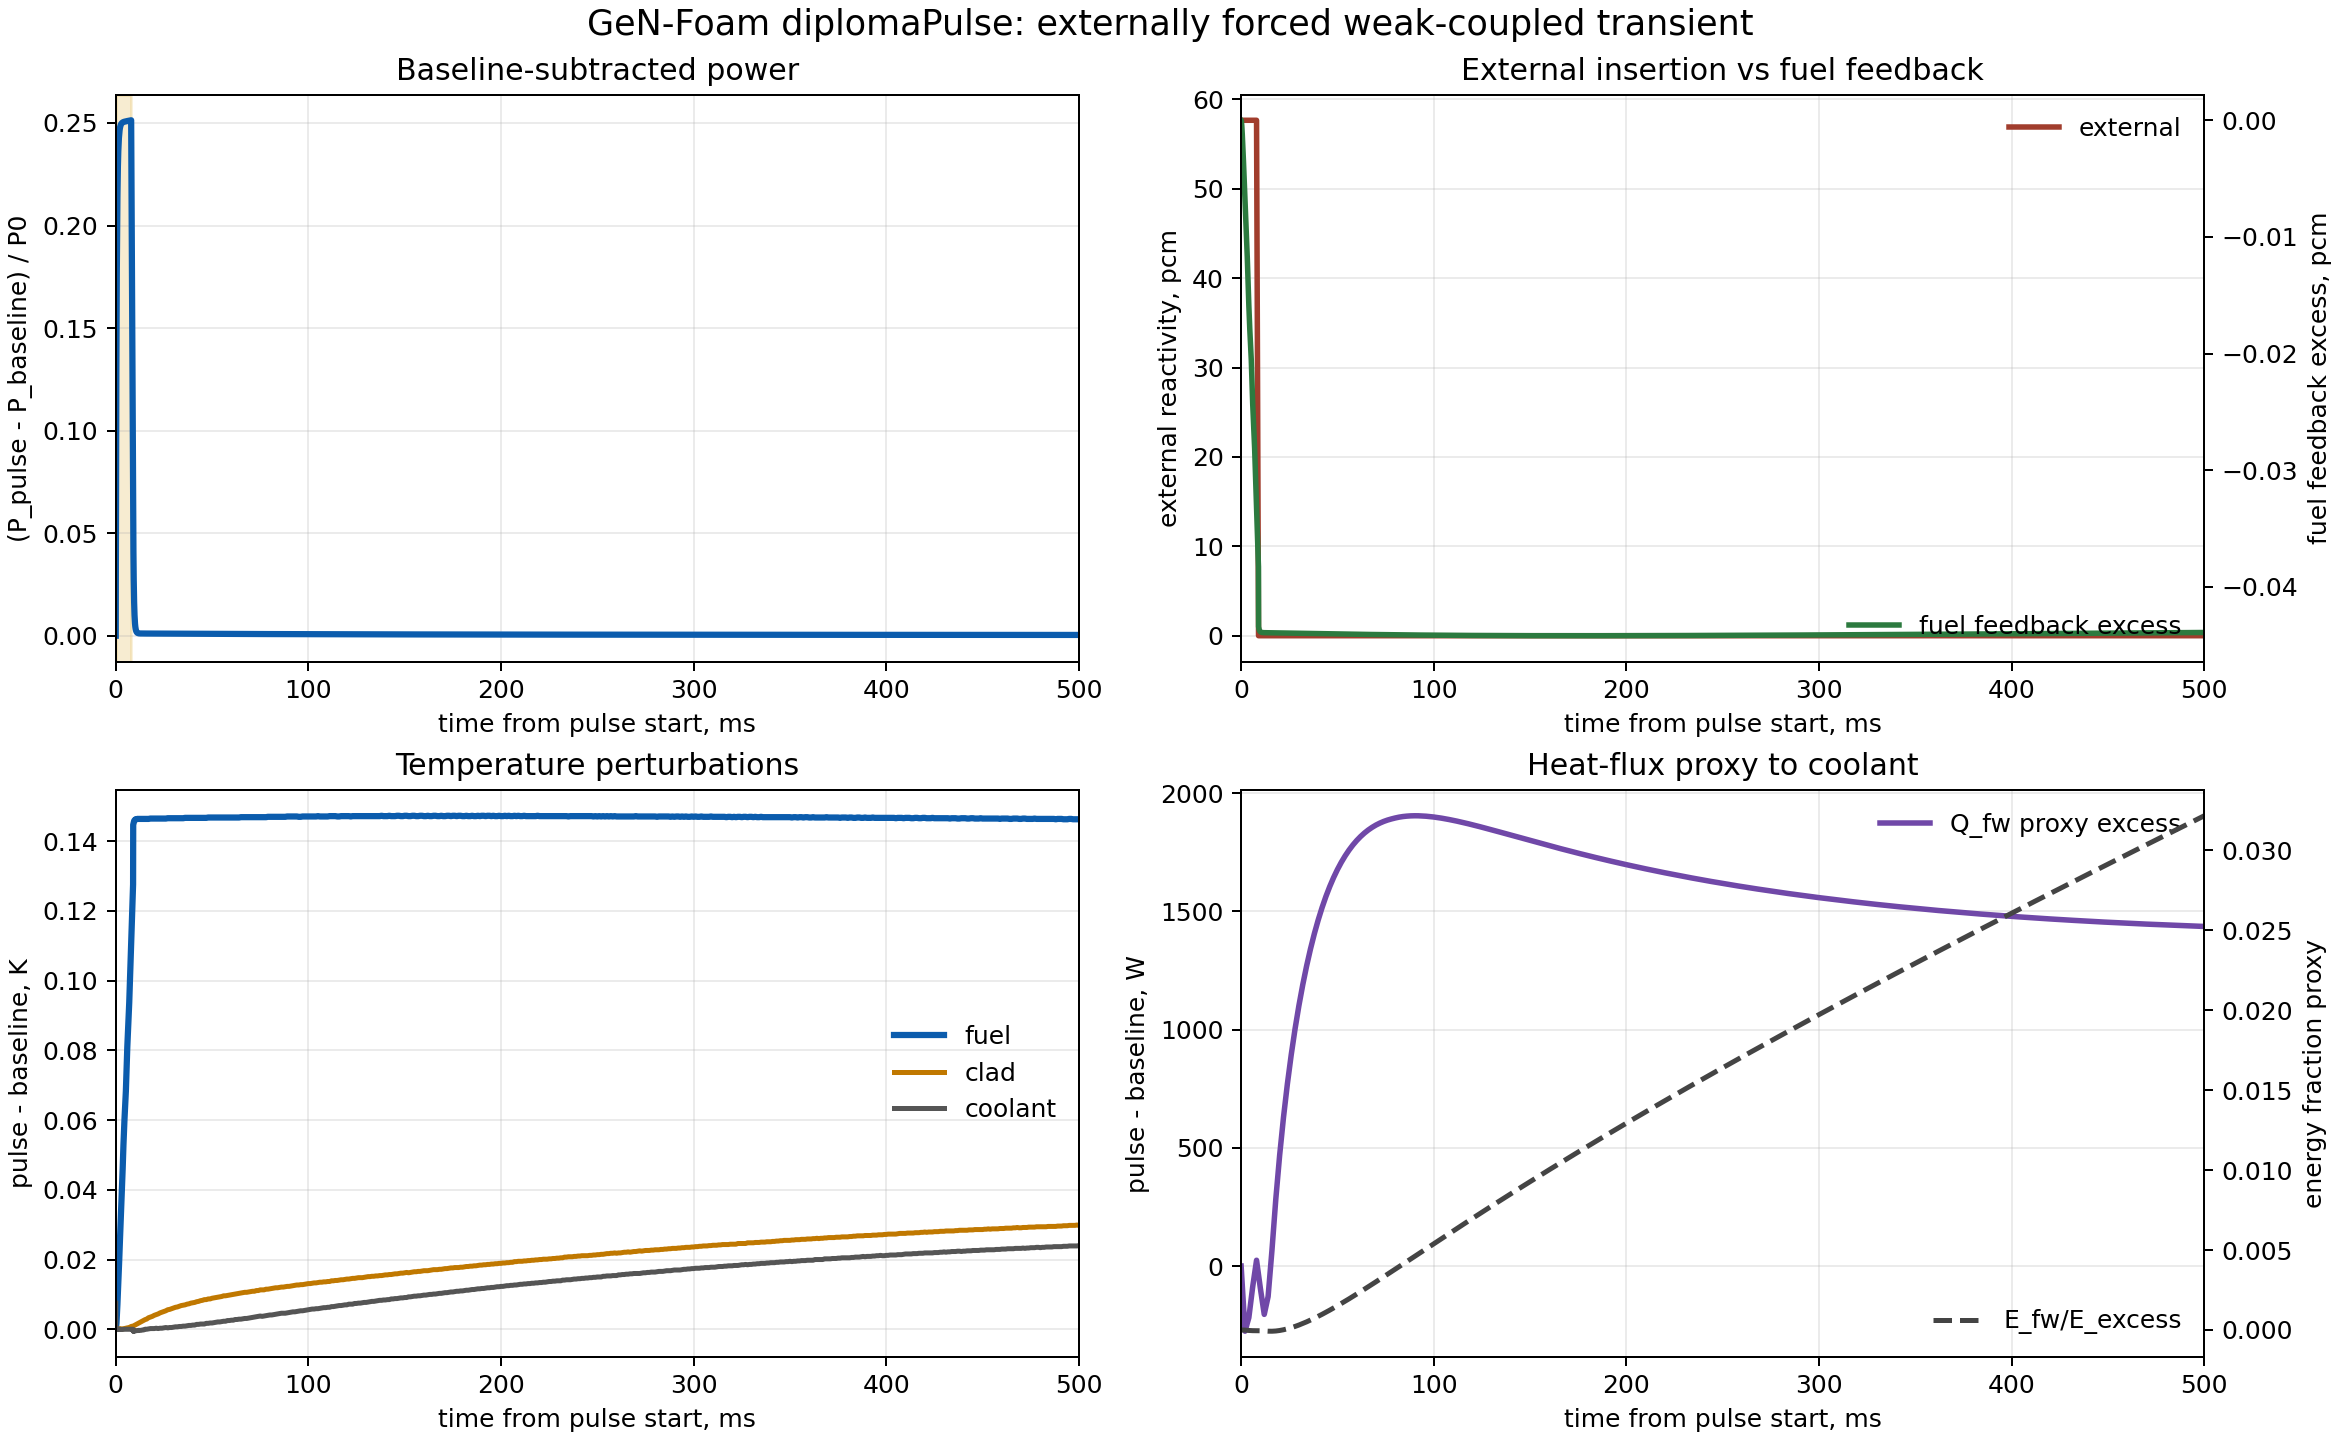
\includegraphics[width=\textwidth]{figures/fig4_genfoam_baseline_subtracted.png}
    \caption{Baseline-subtracted расчёт GeN-Foam. Спад мощности после \(8\,\mathrm{ms}\) связан главным образом с выключением внешней вставки, а не с доплеровским самогашением.}
    \label{fig:genfoamBaselineSubtracted}
\end{figure}

\begin{table}[H]
    \centering
    \caption{Численная диагностика проверочного GeN-Foam расчёта. Тепловой выход вычислен как подсеточный поверхностный интеграл $Q_{fw}=\sum_i q_i''a_{v,i}V_i$ по полю \texttt{heatFlux.structure} модели \texttt{nuclearFuelPin}.}
    \label{tab:genfoamRegimeMetrics}
    \begin{tabular}{>{\raggedright\arraybackslash}p{0.52\textwidth}>{\raggedright\arraybackslash}p{0.33\textwidth}}
        \hline
        Классификация режима & слабосвязанный внешне вынужденный переходный процесс\\
        $\rho_{\mathrm{ext}}^{\max}$ & 57.67 pcm\\
        $P_{\max}/P_0$ & 1.251 при $t=8.0$ ms\\
        $\max|\Delta\rho_{f}|$ & 0.0442 pcm\\
        $\mathcal D=\max|\Delta\rho_f|/\rho_{\mathrm{ext}}^{\max}$ & $7.66\cdot 10^{-4}$\\
        $\max\Delta T_f$ & 0.147 K\\
        $\alpha_{\mathrm{eff}}$ & -0.300 pcm/K\\
        $E_{\text{имп}}$ & 23.87 kJ\\
        $\mathcal W(500\ \mathrm{ms})$ & 0.032\\
        $t_{10\%}$ по $E_w/E_{\text{имп}}$ & ---\\
        \hline
    \end{tabular}
\end{table}


Ключевые числа:
\[
\rho_{\mathrm{ext}}^{\max}=57.67\ \mathrm{pcm},
\qquad
\max|\Delta\rho_f|=0.0442\ \mathrm{pcm},
\]
\[
\mathcal D_{\mathrm{ext}}=
\frac{0.0442}{57.67}
=7.66\cdot10^{-4}.
\]
Следовательно, данный case является externally forced weak-coupled transient. Он не подтверждает центральную доплеровскую модель как режим самогашения; он показывает, что диагностика способна распознать отсутствие сильной доплеровской активации.

В текущей постановке \texttt{nuclearFuelPin} поверхность теплообмена не является явным patch сетки. Поэтому интегральный поток к воде вычисляется как sub-scale поверхностный интеграл
\[
Q_{fw}(t)=\sum_i q_i''(t)a_{v,i}V_i,
\]
где \(q_i''\) берётся из поля \texttt{heatFlux.structure}, а \(a_v=2\alpha_{\mathrm{structure}}/r_{\mathrm{clad}}\). Эта величина пригодна для диагностики теплового канала \(H_{fw}\), но не должна смешиваться с доказательством доплеровского самогашения.

Важно также разделять теоретическую 3D-формулу для \(K_D\) и фактический уровень разрешения GeN-Foam case. Поле доплеровской важности \(D_D(\mathbf r)\) в данном расчёте не восстанавливается как пространственное поле; GeN-Foam используется для интегральной диагностики отклика. Полноценная проверка геометрического функционала \(K_D\) требует либо разрешённого топливного benchmark, либо независимых статических perturbation-расчётов нейтроники при разных температурах топлива.

\section{Идентификация \(H_{fw}\) по диагностической серии}

Для восстановления функций памяти выполнена серия малых импульсов с одинаковой амплитудой внешней реактивности и разными длительностями:
\[
\tau_p=2,\ 4,\ 8,\ 16,\ 32\,\mathrm{ms},
\qquad
t_{\mathrm{end}}=3\,\mathrm{s}.
\]
Входом идентификационной задачи является
\[
u(t)=P_{\mathrm{pulse}}(t)-P_{\mathrm{baseline}}(t),
\]
а выходами являются
\[
y_D(t)=-
\left[
\rho_{f,\mathrm{pulse}}(t)-\rho_{f,\mathrm{baseline}}(t)
\right],
\qquad
y_w(t)=
Q_{fw,\mathrm{pulse}}(t)-Q_{fw,\mathrm{baseline}}(t).
\]
Искомые ядра должны удовлетворять
\[
y_D(t)\approx \int_0^tK_D(t-s)u(s)\,ds,
\qquad
y_w(t)\approx \int_0^tH_{fw}(t-s)u(s)\,ds.
\]
Здесь \(u(t)\) не является независимым управляющим сигналом внешнего эксперимента: мощность сама формируется реактивностью и обратными связями. Для теплового канала это допустимо как post-processing, потому что наблюдаемая excess-мощность является фактическим источником тепла. Для реактивностного канала ситуация хуже: \(y_D\) входит обратно в кинетику мощности, а сам сигнал мал по сравнению с внешней вставкой. Поэтому восстановление \(K_D\) в текущем closed-loop case трактуется только как проверка идентифицируемости, а не как измерение физического ядра.

\begin{table}[H]
    \centering
    \caption{Диагностическая серия GeN-Foam. Первая строка соответствует исходному 500 ms benchmark, остальные строки -- расчётам до \(3\,\mathrm{s}\); поэтому \(\eta_w(0.5s)\) и \(\eta_w(t_f)\) нужно сравнивать отдельно.}
    \label{tab:diagnosticSeries}
    \resizebox{\textwidth}{!}{\begin{tabular}{rrrrrrrrrr}
\hline
$\tau_p$, ms & $E_{\text{имп}}$, kJ & $P_{\max}/P_0$ & $\max|\rho_f|$, pcm & $\mathcal D$ & $E_w(0.5s)$, J & $E_w(t_f)$, J & $\eta_w(0.5s)$ & $\eta_w(t_f)$ & $t_{10\%}$, s\\
\hline
8 & 23.9 & 1.251 & 0.04418 & 0.000766 & 768 & 768 & 0.0322 & 0.0322 & ---\\ 
2 & 7.2 & 1.246 & 0.01023 & 0.000177 & 171 & 977 & 0.0238 & 0.136 & 2.15\\ 
4 & 14.8 & 1.250 & 0.02148 & 0.000372 & 363 & 2.04e+03 & 0.0245 & 0.138 & 2.11\\ 
8 & 30.1 & 1.251 & 0.04418 & 0.000766 & 768 & 4.2e+03 & 0.0255 & 0.14 & 2.07\\ 
16 & 60 & 1.253 & 0.08545 & 0.00148 & 1.5e+03 & 8.22e+03 & 0.025 & 0.137 & 2.12\\ 
32 & 120 & 1.255 & 0.1682 & 0.00292 & 2.91e+03 & 1.62e+04 & 0.0243 & 0.135 & 2.15\\ 
\hline
\end{tabular}
}
\end{table}

Главный результат серии состоит в различии идентифицируемости двух каналов. Тепловой выход \(\Delta Q_{fw}/E_{\mathrm{pulse}}\) и накопленная доля \(E_w/E_{\mathrm{pulse}}\) имеют близкую форму для разных длительностей импульса. Это означает, что в рассматриваемой области тепловой канал хорошо описывается линейным причинным ядром \(H_{fw}\). Реактивностный сигнал \(y_D\) значительно слабее: даже для \(\tau_p=32\,\mathrm{ms}\) \(\mathcal D_{\mathrm{ext}}\) остаётся порядка \(10^{-3}\), поэтому \(K_D\) в данной постановке не восстанавливается надёжно.

\begin{figure}[H]
    \centering
    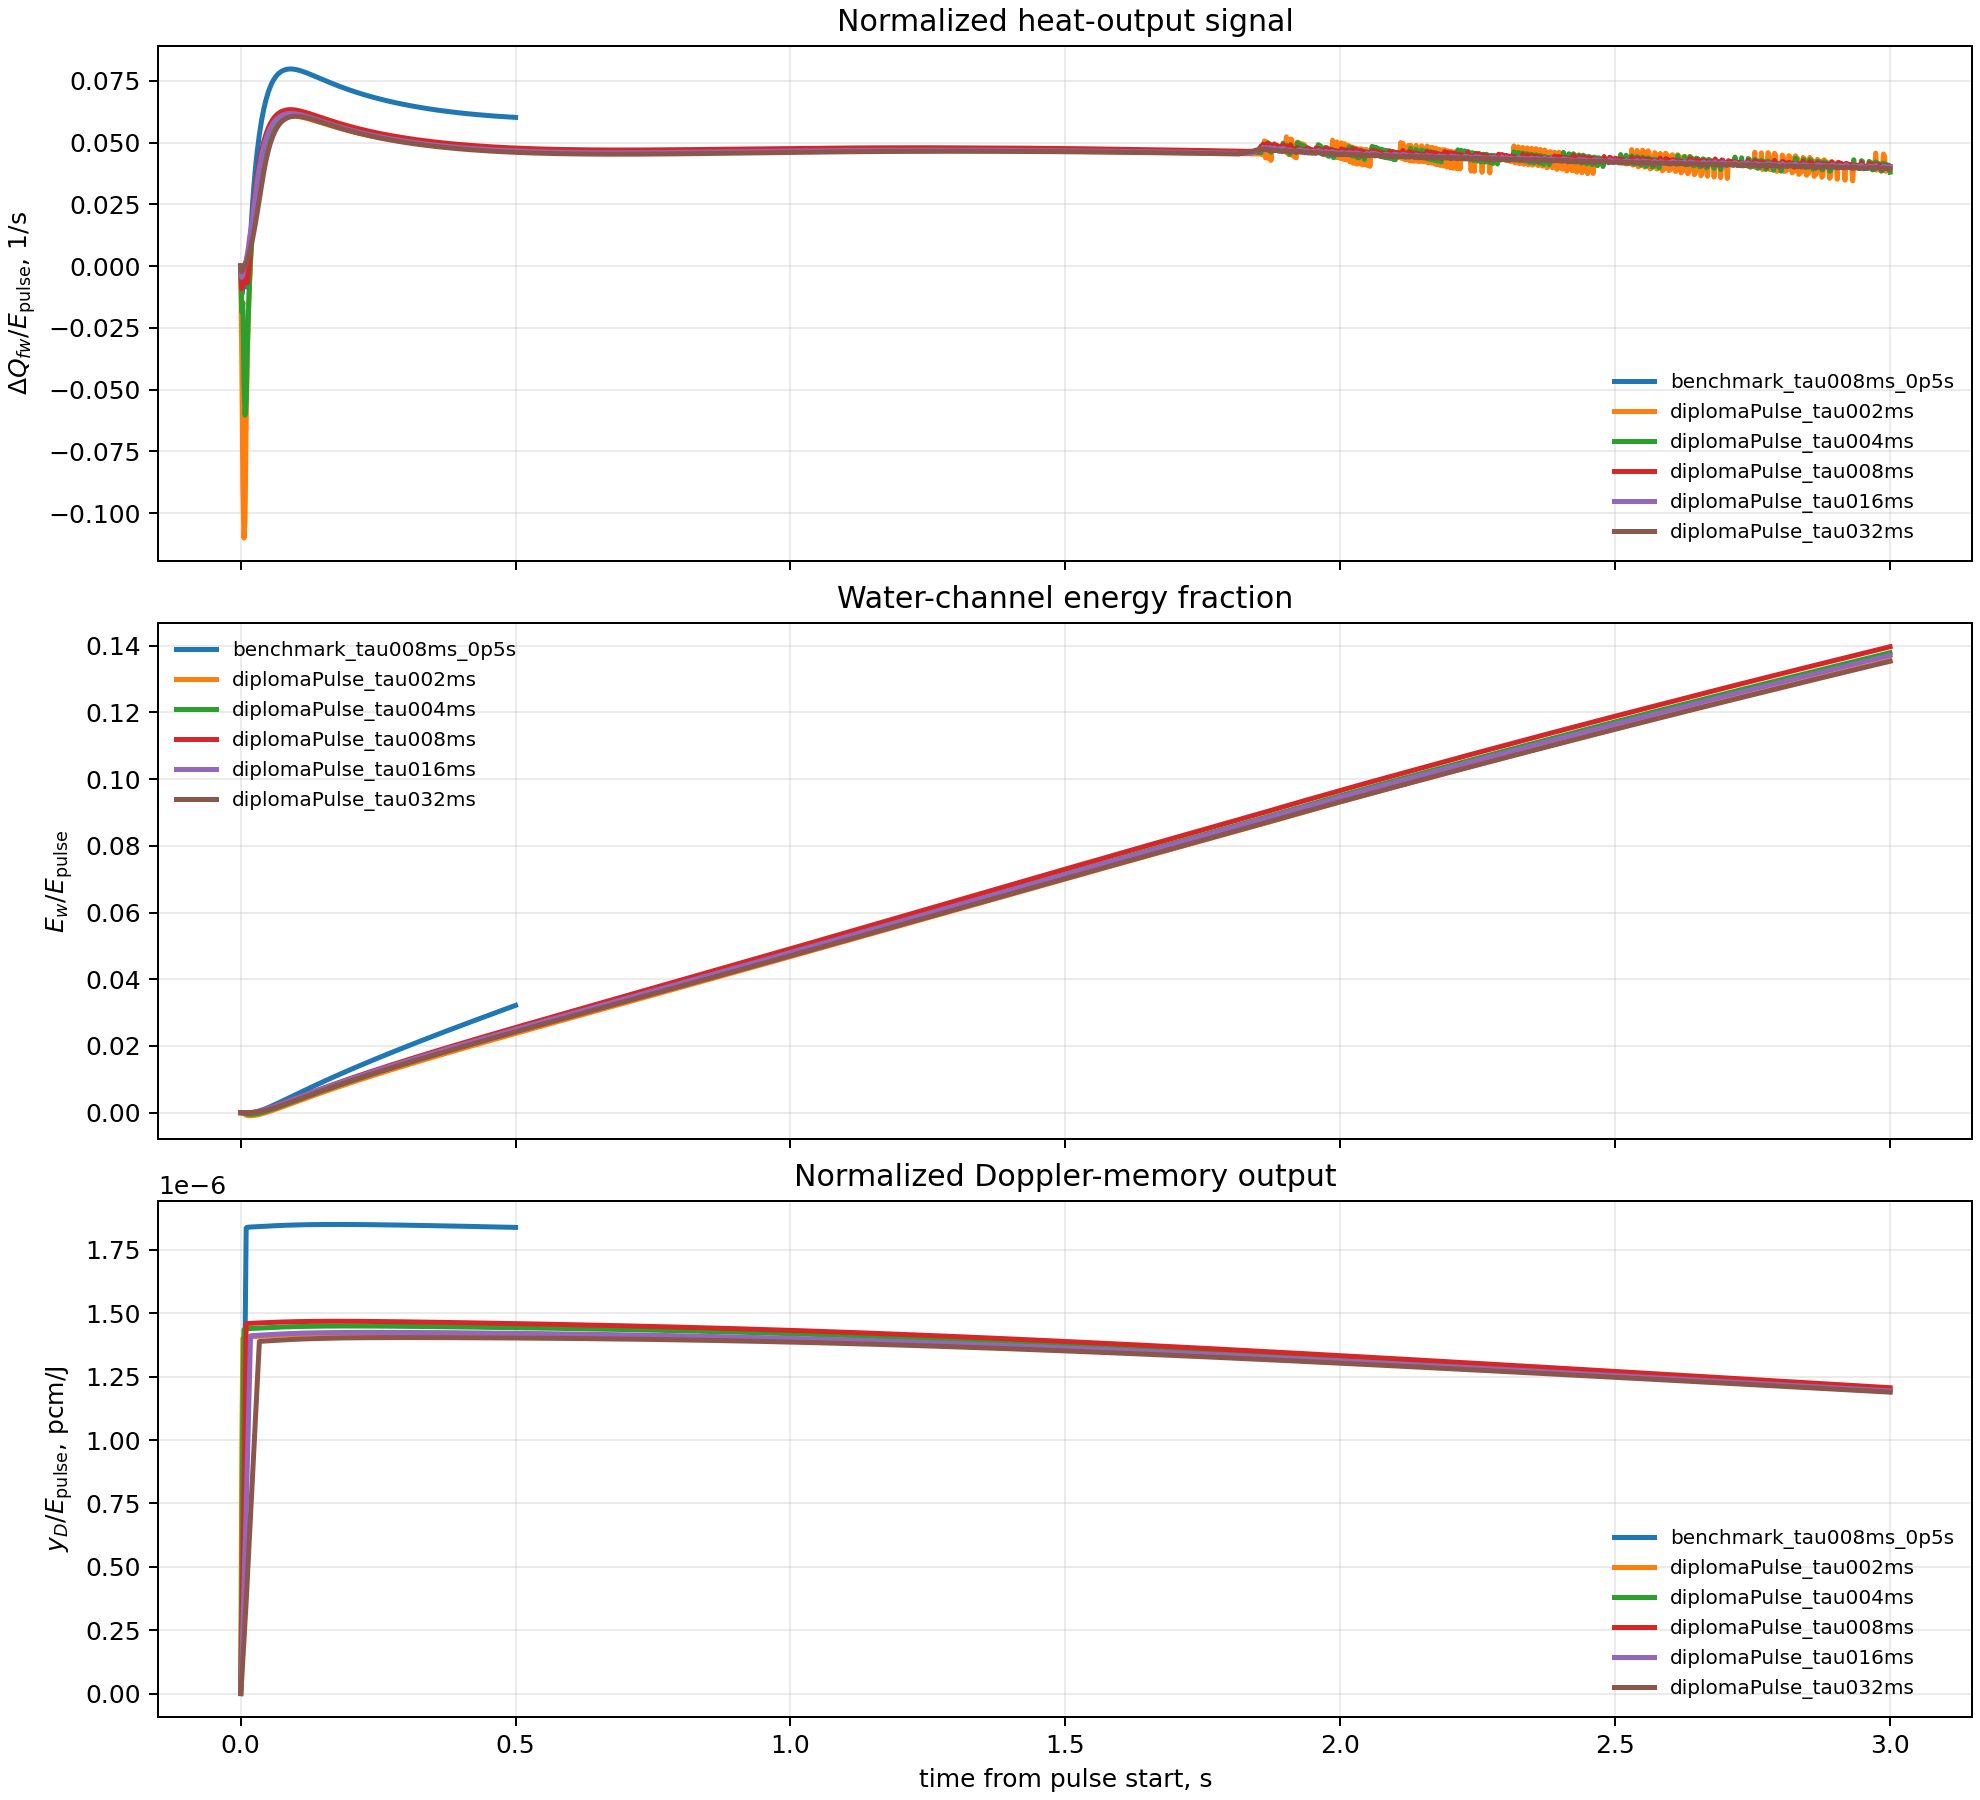
\includegraphics[width=\textwidth]{figures/fig8_diagnostic_normalized_overlays.png}
    \caption{Нормированные отклики диагностической серии. Тепловой канал коллапсирует лучше реактивностного, что указывает на устойчивую идентификацию \(H_{fw}\) и слабую идентифицируемость \(K_D\).}
    \label{fig:diagnosticOverlays}
\end{figure}

На раннем фронте \(Q_{fw}\) возможны малые отрицательные значения после baseline-subtraction. Они не интерпретируются как физический тепловой поток из воды в топливо: для положительного импульса мощности ожидаемое физическое ядро \(H_{fw}\) должно быть неотрицательным. Этот участок отражает чувствительность к вычитанию baseline, sign convention поля \texttt{heatFlux.structure} и начальному согласованию расчёта; поэтому выводы по \(H_{fw}\) опираются прежде всего на нормированную форму после фронта, накопленную энергию и leave-one-out проверку.

На карте режимов диагностическая серия остаётся в области weak forced transient по доплеровскому критерию, но при \(t_{\mathrm{obs}}=3\,\mathrm{s}\) пересекает уровень \(\mathcal W=0.1\). Следовательно, водный канал не отсутствует; он просто имеет длинную память и проявляется позже нейтронного пика.

Рис.~\ref{fig:diagnosticRegimeMap} следует читать с учётом времени наблюдения: исходный benchmark показан при \(t_{\mathrm{obs}}=0.5\,\mathrm{s}\), а диагностические runs -- при \(t_{\mathrm{obs}}=3\,\mathrm{s}\). Поэтому карта иллюстрирует режимную классификацию, но честное сравнение теплового выхода между cases проводится по двум отдельным столбцам таблицы~\ref{tab:diagnosticSeries}: \(\eta_w(0.5s)\) и \(\eta_w(t_f)\).

\begin{figure}[H]
    \centering
    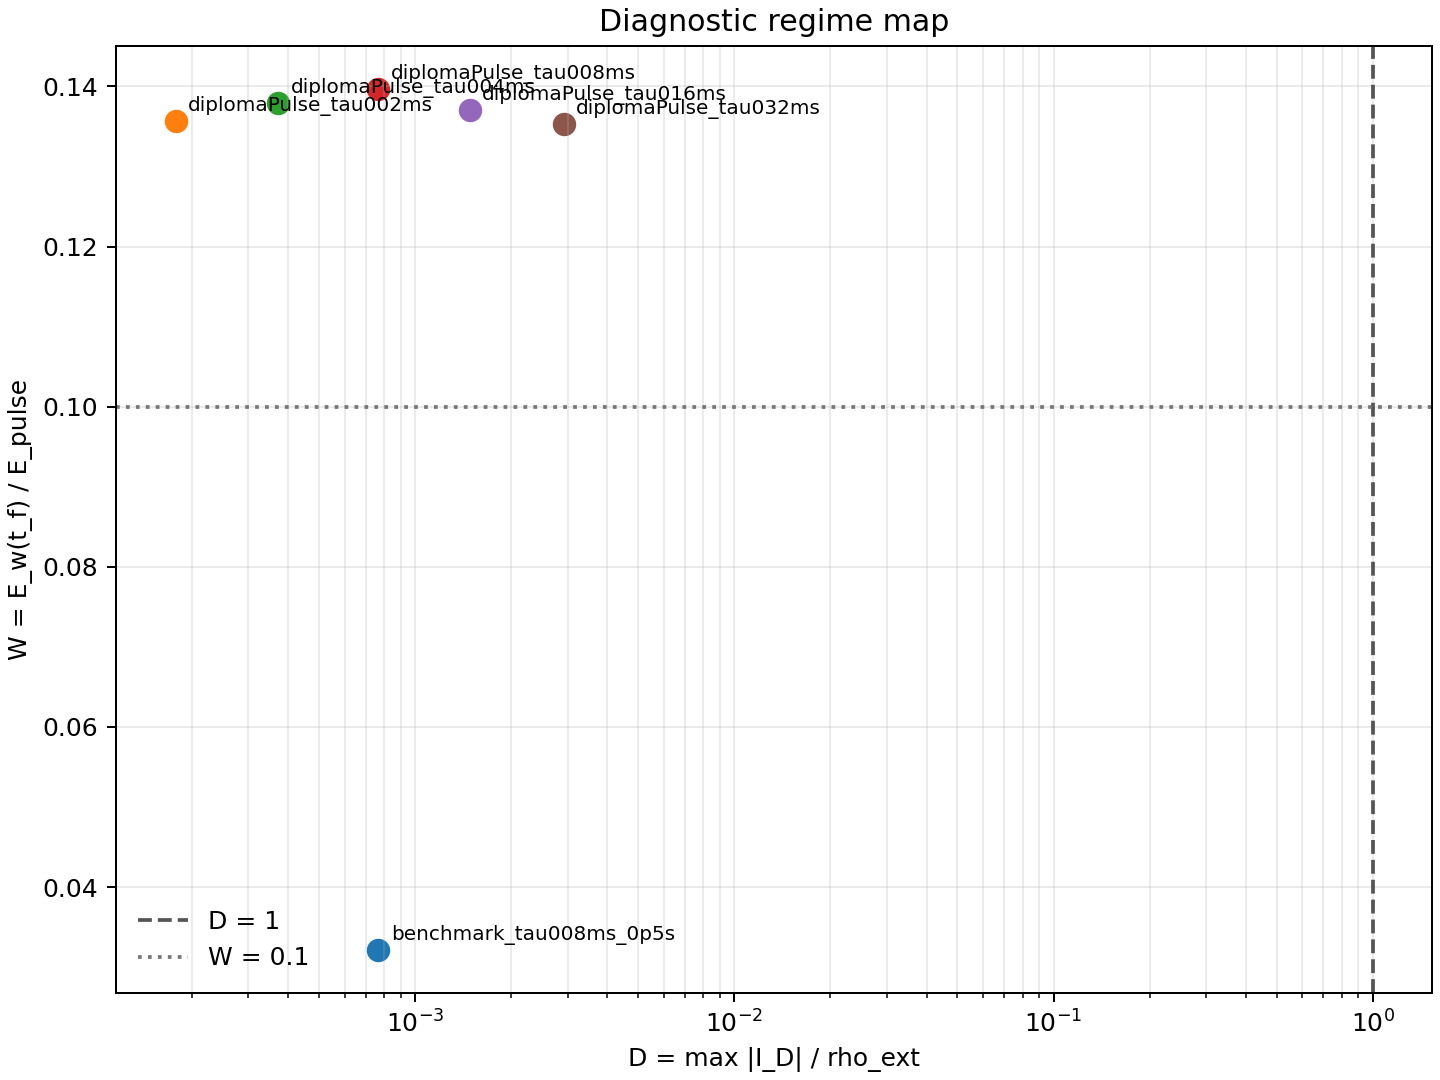
\includegraphics[width=0.82\textwidth]{figures/fig9_diagnostic_regime_map.png}
    \caption{Карта режимов в координатах \(\mathcal D_{\mathrm{ext}}\) и \(\mathcal W(t_{\mathrm{obs}})\). Исходный benchmark имеет \(t_{\mathrm{obs}}=0.5\,\mathrm{s}\), диагностические cases -- \(t_{\mathrm{obs}}=3\,\mathrm{s}\); все точки остаются при \(\mathcal D_{\mathrm{ext}}\ll1\).}
    \label{fig:diagnosticRegimeMap}
\end{figure}

При физической идентификации ядра должны удовлетворять знаковым и энергетическим ограничениям:
\[
H_{fw}(t)\ge0,
\qquad
\int_0^\infty H_{fw}(t)\,dt\le1,
\qquad
K_D(t)\ge0
\]
при записи \(y_D=-\Delta\rho_f\). Поэтому sign-changing fit \(K_D\) не рассматривается как физическое ядро. Он показывает только, что weak-coupled GeN-Foam case не содержит достаточно сильного реактивностного сигнала для устойчивого восстановления \(K_D\).

Совместный fit теплового канала с неотрицательными коэффициентами \(B_j\) и временами
\[
\theta_j=0.05,\ 0.2,\ 1,\ 3,\ 10\,\mathrm{s}
\]
даёт \(R^2\approx0.987\) для \(H_{fw}\). Среднее время памяти fitted kernel составляет около \(8.8\,\mathrm{s}\), что превышает расчётное окно и потому должно пониматься как признак длинного хвоста, а не как окончательно измеренная асимптотическая константа. Для \(K_D\) аналогичная процедура даёт низкое качество восстановления.

\begin{figure}[H]
    \centering
    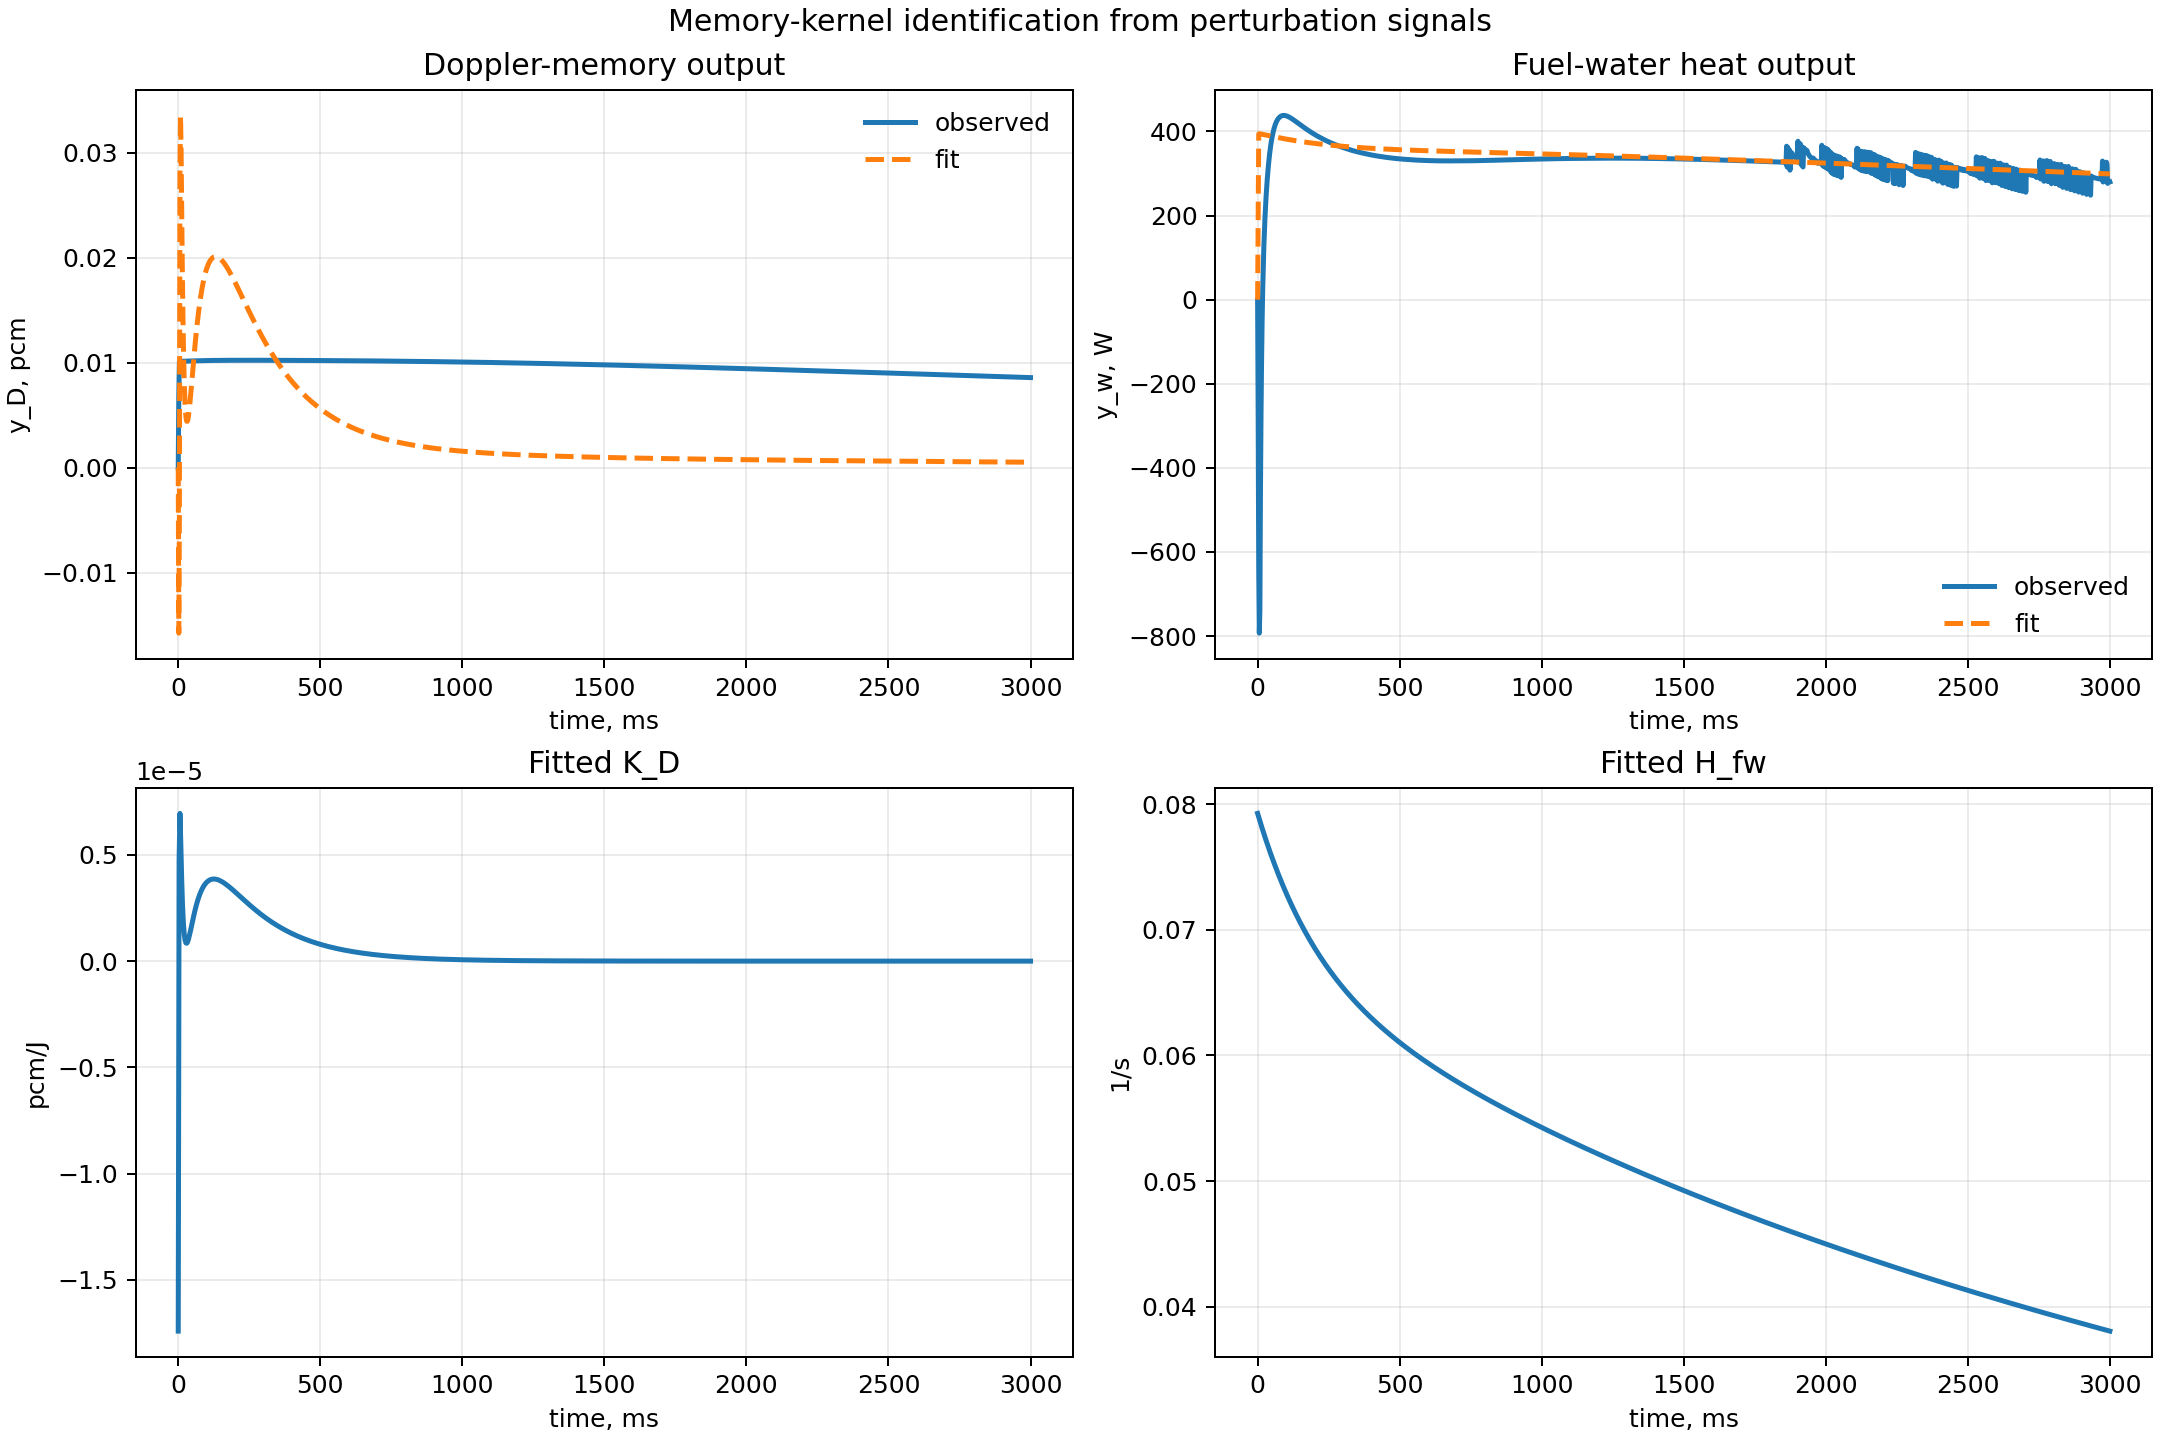
\includegraphics[width=\textwidth]{figures/fig10_kernel_fit.png}
    \caption{Joint fit экспоненциальных ядер: \(H_{fw}\) воспроизводится существенно лучше, чем \(K_D\). Sign-changing fit \(K_D\) показан как диагностика неидентифицируемости, а не как физическое реактивностное ядро.}
    \label{fig:kernelFit}
\end{figure}

Для проверки переносимости используется leave-one-out схема: ядро \(H_{fw}\) подбирается по четырём длительностям импульса и предсказывает пятую. Такая проверка важнее визуального совпадения, потому что показывает, что тепловой канал не просто подогнан под один график, а переносится между cases.

\begin{figure}[H]
    \centering
    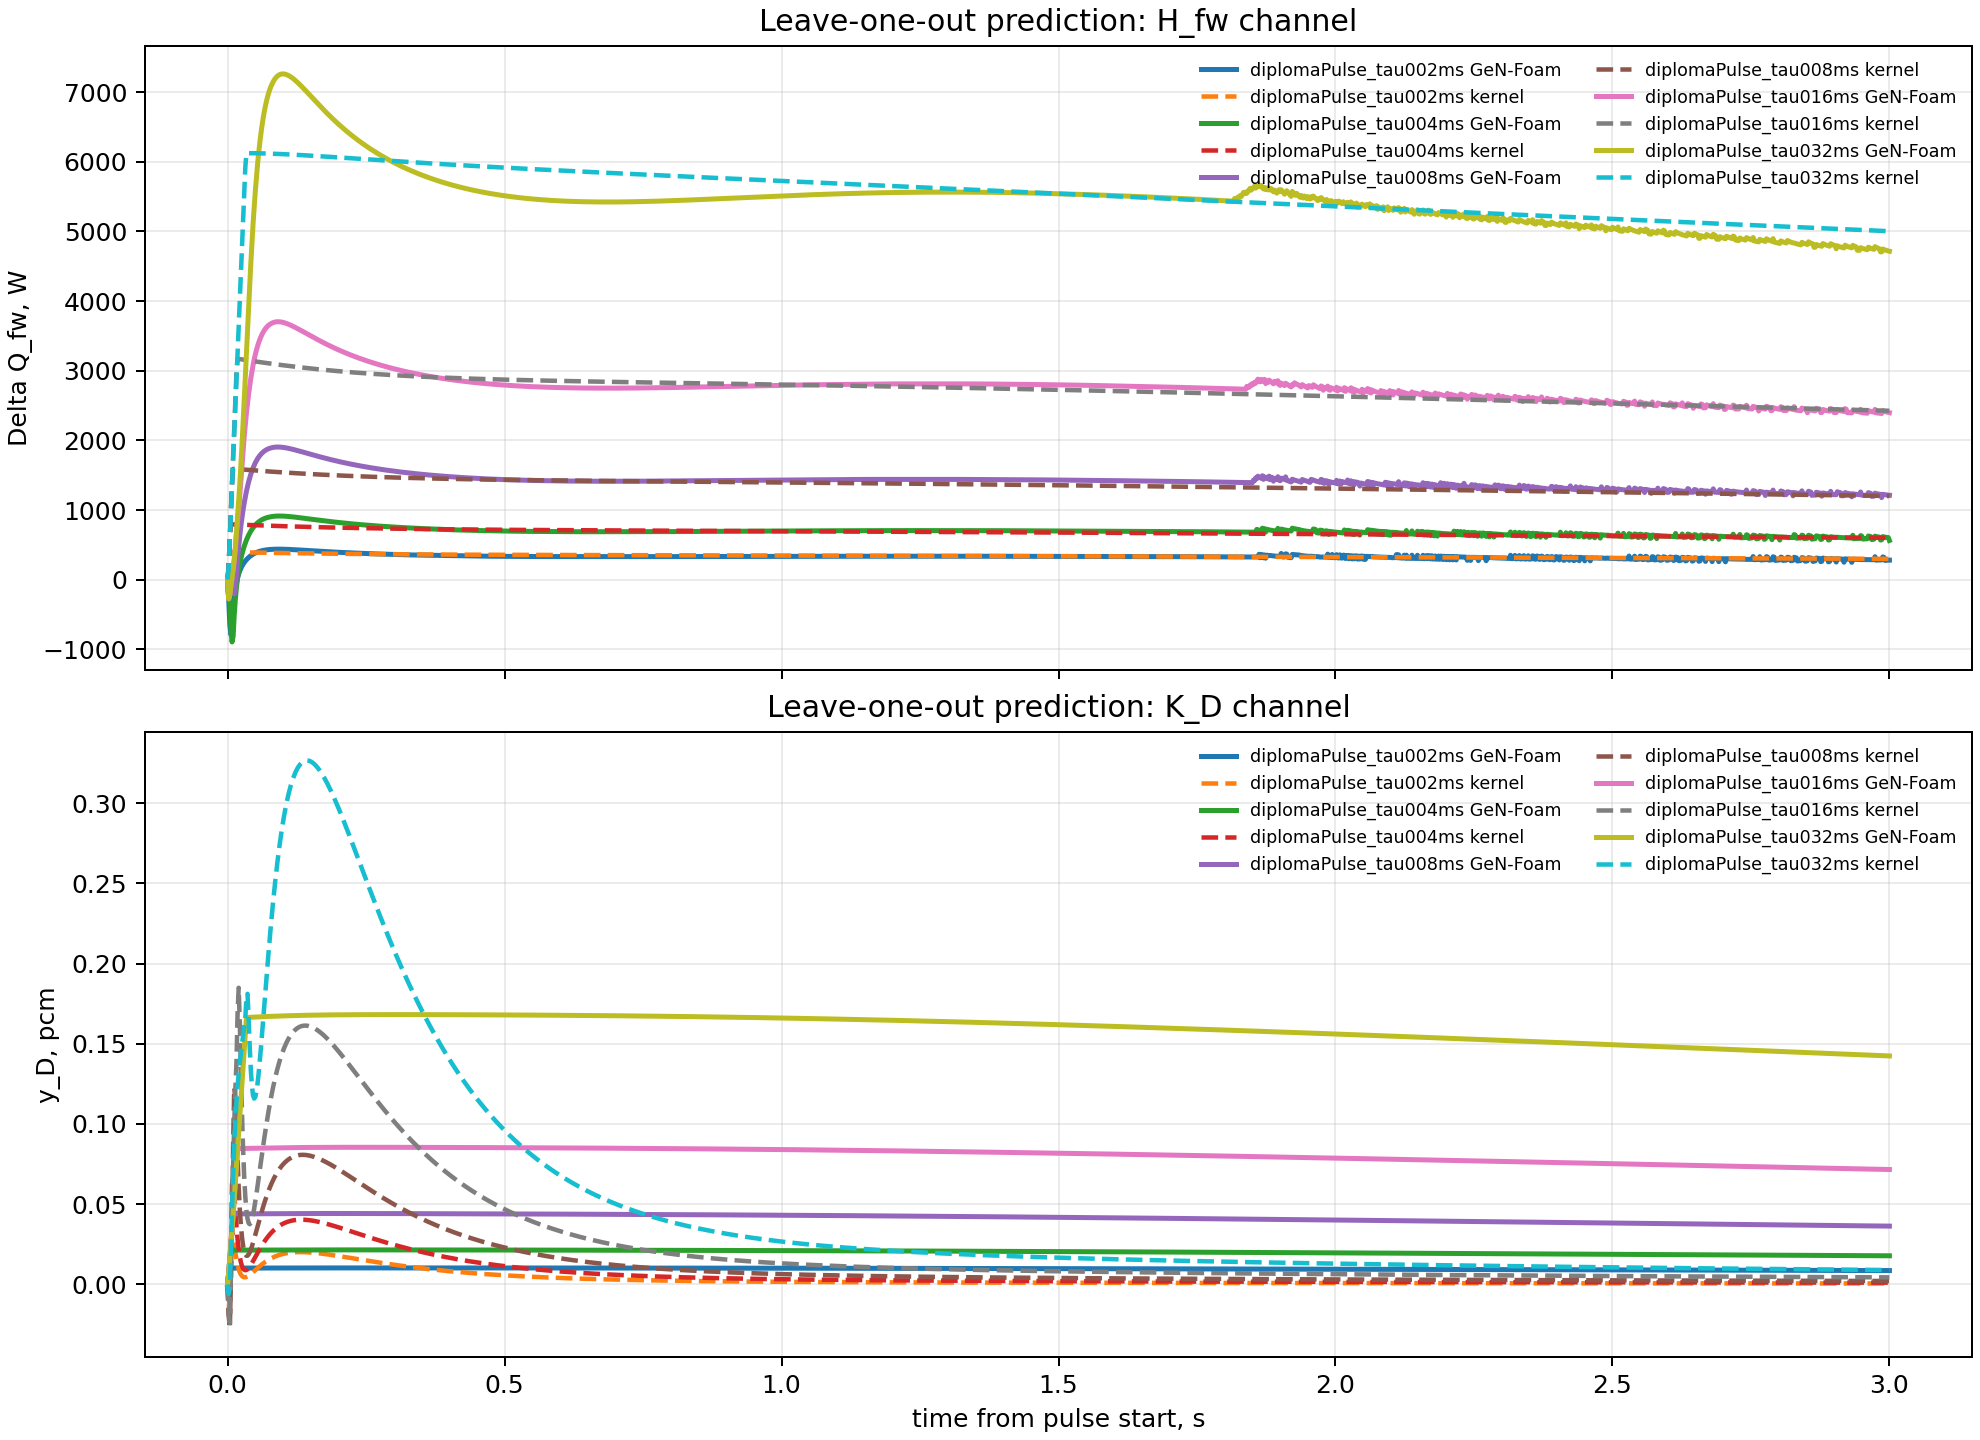
\includegraphics[width=\textwidth]{figures/fig11_leave_one_out_prediction.png}
    \caption{Leave-one-out prediction. Тепловой канал воспроизводит интегральные энергии лучше, чем ранний фронт; реактивностный канал остаётся слабо предсказуемым.}
    \label{fig:leaveOneOutPrediction}
\end{figure}

\section{Обсуждение}

Полученные результаты требуют аккуратной интерпретации. Теоретическая модель описывает режим, в котором твэл может работать как доплеровский элемент памяти: история мощности создаёт \(I_D=K_D*P\), а затем отрицательная реактивность ограничивает дальнейший рост мощности. Reduced-модель показывает такой целевой режим качественно. Однако GeN-Foam benchmark относится к другой области параметров: внешняя вставка реактивности доминирует, а топливная обратная связь мала.

Именно поэтому основной численный вывод состоит не в доказательстве самогашения, а в классификации режима. При
\[
\mathcal D_{\mathrm{ext}}=7.66\cdot10^{-4}
\]
текущий benchmark не может считаться доплеровски активным. Это ограничение не обесценивает расчёт: оно показывает, что предложенная диагностика различает целевой Doppler-active режим и слабосвязанный forced transient.

Положительный результат GeN-Foam части относится к тепловому каналу. Серия малых импульсов показывает, что \(H_{fw}\) может быть идентифицирован как линейное причинное ядро. При этом тепловая память оказывается секундной, а не миллисекундной. Поэтому в финальной версии работы важно не утверждать универсально \(\tau_H\sim10\)--\(100\,\mathrm{ms}\), а разделять идеализированную диффузионную оценку и effective \(H_{fw}\), полученный в конкретной sub-scale модели GeN-Foam.

Реактивностное ядро \(K_D\) в текущей постановке не идентифицируется надёжно. Корректная формулировка результата такова: \(H_{fw}\) восстановлено по диагностической серии, а для \(K_D\) получена только оценка слабой доплеровской активации. Для перехода к полноценной проверке \(K_D\) нужен отдельный Doppler-active benchmark, например controlled reduced model
\[
\rho_{\mathrm{eff}}(t)=
\rho_0-K_D*P,
\]
в котором \(\mathcal D_{\mathrm{ext}}\sim1\) и самогашение действительно формируется топливом.

Отдельно следует отметить численный noise floor по \(\rho_f\). В выполненной обработке есть только оценка гладкости самого \(y_D(t)\), но нет строгого шума из повторных no-pulse расчётов или независимого pre-pulse окна. Поэтому малость \(\max|\Delta\rho_f|=0.0442\,\mathrm{pcm}\) рассматривается как основание для классификации режима, но не как достаточная база для точного восстановления формы \(K_D(t)\).

Число \(\alpha_{\mathrm{eff}}=-0.300\,\mathrm{pcm/K}\), приведённое в таблице диагностики, также не следует трактовать как независимый статический коэффициент материала. В данной работе это transient-оценка по малому сигналу. Для самостоятельной верификации доплеровской физики требуются статические perturbation runs при \(T_f=T_0+\Delta T\) и независимое вычисление \(\Delta\rho/\Delta T\). В перспективе для этого подходит, например, OpenMC с windowed multipole representation для on-the-fly Doppler broadening \cite{OpenMCCrossSections}; в текущем тексте OpenMC рассматривается именно как возможный источник статических данных, а не как выполненная часть численного исследования.

Энергетическая интерпретация \(\mathcal W(3\,\mathrm{s})\approx0.135\)--\(0.140\) также ограничена уровнем доступных данных. Эта величина означает, что за \(3\,\mathrm{s}\) в sub-scale водный канал перешла указанная доля excess-энергии. Остальная энергия не считается потерянной: она остаётся в тепловой инерции топлива, оболочки, теплоносителя и численном остатке баланса. Полное закрытие баланса требует отдельной таблицы \(E_{\mathrm{pulse}}=\Delta E_f+\Delta E_{\mathrm{clad}}+\Delta E_c+E_w+\varepsilon\), которая выходит за рамки выполненной обработки.

\section{Заключение}

В работе построена двухканальная модель памяти твэла. История мощности преобразуется в два причинных функционала:
\[
I_D(t)=\int_0^tK_D(t-s)P(s)\,ds,
\qquad
Q_{fw}(t)=\int_0^tH_{fw}(t-s)P(s)\,ds.
\]
Первый функционал описывает доплеровскую реактивностную память топлива, второй -- задержанный тепловой поток в воду.

Построено геометрическое выражение для \(K_D\), связывающее форму энерговыделения, тепловую функцию Грина и поле доплеровской важности. Аналогично сформулировано ядро \(H_{fw}\), определяемое граничным тепловым функционалом на поверхности теплообмена. Введены диагностические параметры \(\mathcal D_{\mathrm{ext}}\), \(\mathcal D_\beta\) и \(\mathcal W(t_{\mathrm{obs}})\), позволяющие различать доплеровски активный режим и weak-coupled forced transient.

GeN-Foam benchmark классифицирован как слабосвязанный внешне вынужденный переходный процесс:
\[
\rho_{\mathrm{ext}}^{\max}=57.67\,\mathrm{pcm},
\qquad
\max|\Delta\rho_f|=0.0442\,\mathrm{pcm},
\qquad
\mathcal D_{\mathrm{ext}}=7.66\cdot10^{-4}.
\]
Следовательно, этот расчёт не доказывает доплеровское самогашение, но служит проверкой диагностики.

По диагностической серии импульсов \(\tau_p=2,\ 4,\ 8,\ 16,\ 32\,\mathrm{ms}\) показано, что тепловой канал \(H_{fw}\) идентифицируется устойчиво: нормированные тепловые отклики имеют близкую форму, joint fit даёт \(R^2\approx0.987\), а leave-one-out prediction подтверждает переносимость ядра. При этом к \(3\,\mathrm{s}\) в водный канал уходит около \(13.5\)--\(14.0\%\) excess-энергии, что указывает на секундную память теплового канала в данной GeN-Foam постановке.

Не доказаны в текущем GeN-Foam case сильное доплеровское самогашение, надёжное восстановление \(K_D\) и участие воды в формировании пика мощности. Эти ограничения являются частью результата: предложенная модель не только описывает целевой режим памяти твэла, но и даёт диагностику, показывающую, когда конкретный расчёт этому режиму не соответствует.

\newpage
\section{Список литературы}
\begin{thebibliography}{15}
    \bibitem{DuderstadtHamilton1976}
    Duderstadt J. J., Hamilton L. J. \textit{Nuclear Reactor Analysis}. Wiley, 1976.

    \bibitem{NRCFeedback2012}
    U.S. Nuclear Regulatory Commission. \textit{Module 10: Power Reactor Feedback Effects. Rev. 01}. 2012. URL: \href{https://www.nrc.gov/docs/ML1214/ML12142A130.pdf}{nrc.gov/docs/ML1214/ML12142A130.pdf}.

    \bibitem{DOEGeneralTechnicalBase2013}
    U.S. Department of Energy. \textit{General Technical Base Qualification Standard Reference Guide}. 2012. URL: \href{https://www.energy.gov/sites/prod/files/2013/10/f4/QSR-GeneralTechnicalBase.pdf}{energy.gov/sites/prod/files/2013/10/f4/QSR-GeneralTechnicalBase.pdf}.

    \bibitem{OpenMCCrossSections}
    OpenMC Documentation. \textit{Cross Section Representations}. URL: \href{https://docs.openmc.org/en/stable/methods/cross_sections.html}{docs.openmc.org/en/stable/methods/cross\_sections.html}.

    \bibitem{MOOSEHeatTransfer}
    MOOSE Framework. \textit{Heat Transfer Module}. URL: \href{https://mooseframework.inl.gov/modules/heat_transfer/}{mooseframework.inl.gov/modules/heat\_transfer}.

    \bibitem{OpenFOAMSolvers}
    OpenFOAM Documentation. \textit{Standard Solvers}. URL: \href{https://www.openfoam.com/documentation/user-guide/a-reference/a.1-standard-solvers}{openfoam.com/documentation/user-guide/a-reference/a.1-standard-solvers}.

    \bibitem{GeNFoam2015}
    Fiorina C., Clifford I., Aufiero M., Mikityuk K. GeN-Foam: A Novel OpenFOAM Based Multi-Physics Solver for 2D/3D Transient Analysis of Nuclear Reactors // \textit{Nuclear Engineering and Design}. 2015. Vol. 294. P. 24--37. DOI: \href{https://doi.org/10.1016/j.nucengdes.2015.05.035}{10.1016/j.nucengdes.2015.05.035}.

    \bibitem{foamForNuclear2026}
    Nervi G., Guilbaud T., Fiorina C., Hursin M., Scolaro A. foamForNuclear: A Unified OpenFOAM Multi-Physics Platform for Nuclear Applications // \textit{Progress in Nuclear Energy}. 2026. Vol. 193. Article 106250. DOI: \href{https://doi.org/10.1016/j.pnucene.2026.106250}{10.1016/j.pnucene.2026.106250}.
\end{thebibliography}

\end{document}
